%%%%%%%%%%%%%%%%%%%%%%%%%%%%%%%%%%%%%%%%%
% Proceedings of the National Academy of Sciences (PNAS)
% LaTeX Template
% Version 1.0 (19/5/13)
%
% This template has been downloaded from:
% http://www.LaTeXTemplates.com
%
% Original author:
% The PNAStwo class was created and is owned by PNAS:
% http://www.pnas.org/site/authors/LaTex.xhtml
% This template has been modified from the blank PNAS template to include
% examples of how to insert content and drastically change commenting. The
% structural integrity is maintained as in the original blank template.
%
% Original header:
%% PNAStmpl.tex
%% Template file to use for PNAS articles prepared in LaTeX
%% Version: Apr 14, 2008
%
%%%%%%%%%%%%%%%%%%%%%%%%%%%%%%%%%%%%%%%%%
%----------------------------------------------------------------------------------------
%	PACKAGES AND OTHER DOCUMENT CONFIGURATIONS
%----------------------------------------------------------------------------------------

%------------------------------------------------
% BASIC CLASS FILE
%------------------------------------------------

%% PNAStwo for two column articles is called by default.
%% Uncomment PNASone for single column articles. One column class
%% and style files are available upon request from pnas@nas.edu.

%\documentclass{pnasone}
\documentclass{pnastwo}

%------------------------------------------------
% POSITION OF TEXT
%------------------------------------------------

%% Changing position of text on physical page:
%% Since not all printers position
%% the printed page in the same place on the physical page,
%% you can change the position yourself here, if you need to:

%\advance\voffset -.5in % Minus dimension will raise the printed page on the 
                         %  physical page; positive dimension will lower it.

%% You may set the dimension to the size that you need.

%------------------------------------------------
% GRAPHICS STYLE FILE
%------------------------------------------------

%% Requires graphics style file (graphicx.sty), used for inserting
%% .eps/image files into LaTeX articles.
%% Note that inclusion of .eps files is for your reference only;
%% when submitting to PNAS please submit figures separately.

%% Type into the square brackets the name of the driver program 
%% that you are using. If you don't know, try dvips, which is the
%% most common PC driver, or textures for the Mac. These are the options:

% [dvips], [xdvi], [dvipdf], [dvipdfm], [dvipdfmx], [pdftex], [dvipsone],
% [dviwindo], [emtex], [dviwin], [pctexps], [pctexwin], [pctexhp], [pctex32],
% [truetex], [tcidvi], [vtex], [oztex], [textures], [xetex]


%------------------------------------------------
% OPTIONAL POSTSCRIPT FONT FILES
%------------------------------------------------

%% PostScript font files: You may need to edit the PNASoneF.sty
%% or PNAStwoF.sty file to make the font names match those on your system. 
%% Alternatively, you can leave the font style file commands commented out
%% and typeset your article using the default Computer Modern 
%% fonts (recommended). If accepted, your article will be typeset
%% at PNAS using PostScript fonts.

% Choose PNASoneF for one column; PNAStwoF for two column:
%\usepackage{PNASoneF}
%\usepackage{PNAStwoF}

%------------------------------------------------
% ADDITIONAL OPTIONAL STYLE FILES
%------------------------------------------------

%% The AMS math files are commonly used to gain access to useful features
%% like extended math fonts and math commands.
%\usepackage{multirow}
%\usepackage{caption}
%\usepackage{subcaption}
%\usepackage{etex}
%\usepackage{color}
%\usepackage[usenames,dvipsnames,svgnames,table]{xcolor}
%\usepackage[usenames,dvipsnames]{xcolor}
%\usepackage{tikz}
%\usetikzlibrary{decorations.shapes}
\usepackage{amssymb,amsfonts,amsmath}
%\usepackage{xspace}
\usepackage[perpage,symbol]{footmisc}
\newcommand{\dictionary}{\ensuremath{\mathcal{D}}\xspace}

%\usepackage{hyperref}
%\usepackage{soul}

%------------------------------------------------
% OPTIONAL MACRO FILES
%------------------------------------------------

%% Insert self-defined macros here.
%% \newcommand definitions are recommended; \def definitions are supported

%\newcommand{\mfrac}[2]{\frac{\displaystyle #1}{\displaystyle #2}}
%\def\s{\sigma}

%------------------------------------------------
% DO NOT EDIT THIS SECTION
%------------------------------------------------

%% For PNAS Only:
\contributor{Submitted to Proceedings of the National Academy of Sciences of the United States of America}
\url{www.pnas.org/cgi/doi/10.1073/pnas.0709640104}
\copyrightyear{2008}
\issuedate{Issue Date}
\volume{Volume}
\issuenumber{Issue Number}

%----------------------------------------------------------------------------------------

\begin{document}

%----------------------------------------------------------------------------------------
%	TITLE AND AUTHORS
%----------------------------------------------------------------------------------------

\title{Nonliteral understanding of number words} % For titles, only capitalize the first letter

%------------------------------------------------

%% Enter authors via the \author command.  
%% Use \affil to define affiliations.
%% (Leave no spaces between author name and \affil command)

%% Note that the \thanks{} command has been disabled in favor of
%% a generic, reserved space for PNAS publication footnotes.

%% \author{<author name>
%% \affil{<number>}{<Institution>}} One number for each institution.
%% The same number should be used for authors that
%% are affiliated with the same institution, after the first time
%% only the number is needed, ie, \affil{number}{text}, \affil{number}{}
%% Then, before last author ...
%% \and
%% \author{<author name>
%% \affil{<number>}{}}

%% For example, assuming Garcia and Sonnery are both affiliated with
%% Universidad de Murcia:
%% \author{Roberta Graff\affil{1}{University of Cambridge, Cambridge,
%% United Kingdom},
%% Javier de Ruiz Garcia\affil{2}{Universidad de Murcia, Bioquimica y Biologia
%% Molecular, Murcia, Spain}, \and Franklin Sonnery\affil{2}{}}

\author{Justine T. Kao\affil{1}{Stanford University},
Jean Wu,\affil{1}{}
Leon Bergen\affil{2}{MIT}
\and
Noah D. Goodman\affil{1}{}}

\contributor{Submitted to Proceedings of the National Academy of Sciences
of the United States of America}

%----------------------------------------------------------------------------------------

\maketitle % The \maketitle command is necessary to build the title page

\begin{article}

%----------------------------------------------------------------------------------------
%	ABSTRACT, KEYWORDS AND ABBREVIATIONS
%----------------------------------------------------------------------------------------

\begin{abstract}
One of the most puzzling and important facts about communication is that people do not always mean what they say; speakers often use imprecise, exaggerated, or otherwise literally false descriptions to communicate experiences and attitudes. Here we focus on the nonliteral interpretation of number words, in particular hyperbole (interpreting unlikely numbers as exaggerated and conveying affect) and pragmatic halo (interpreting round numbers imprecisely). We provide a computational model of number interpretation as social inference regarding the communicative goal, meaning, and affective subtext of an utterance. We show that our model predicts humans' interpretation of number words with high accuracy. Our model is the first to incorporate empirically measured background knowledge and principles of communication to quantitatively predict hyperbolic and pragmatic halo effects in number interpretation.
This modeling framework provides a unified approach to nonliteral language understanding more generally.\\\\Significance statement: Human communication is rife with nonliteral language, ranging from metaphor to irony to hyperbole. How do people go so far beyond the literal meaning of an utterance to infer the speaker's intended meaning? We present a computational model that understands hyperbolic and other nonliteral uses of number words (e.g. ``That watch costs ten thousand dollars"). Our model integrates empirically measured background knowledge, principles of communication, and reasoning about communicative goals to explain the computational basis of nonliteral language understanding. This framework sheds light on the nature of communication, marking a significant advancement in the flexibility and richness of formal models of language understanding.
\end{abstract}

%------------------------------------------------

%------------------------------------------------

%% Optional for entering abbreviations, separate the abbreviation from
%% its definition with a comma, separate each pair with a semicolon:
%% for example:
%% \abbreviations{SAM, self-assembled monolayer; OTS,
%% octadecyltrichlorosilane}

% \abbreviations{}
%\abbreviations{IR, Incongruity Resolution}

%----------------------------------------------------------------------------------------
%	PUBLICATION CONTENT
%----------------------------------------------------------------------------------------

%% The first letter of the article should be drop cap: \dropcap{} e.g.,
%\dropcap{I}n this article we study the evolution of ''almost-sharp'' fronts
%\section{Significance statement}
%Human communication is rife with nonliteral language, ranging from metaphor to irony to hyperbole. How do people go so far beyond the literal meaning of an utterance to infer the speaker�s intended meaning? We present a computational model that understands hyperbolic and other nonliteral uses of number words (e.g. �That watch cost ten thousand dollars.�) We show that our model predicts humans� interpretation of hyperbole and its rhetorical effects with high accuracy. Our model integrates background knowledge, principles of communication, and reasoning about communicative goals to explain the computational basis of nonliteral language understanding. This framework sheds light on the nature of communication, marking a significant advancement in the flexibility and richness of formal models of language understanding.

\keywords{Pragmatics | Language understanding | Computational modeling} % When adding keywords, separate each term with a straight line: |
\section{Introduction}

\dropcap{I}magine a friend describing a new restaurant where she recently dined. Your friend says, ``It took 30 minutes to get a table." You are likely to interpret this to mean she waited approximately 30 minutes. Suppose she says: ``It took 32 minutes to get a table." You are more likely to interpret this to mean exactly 32 minutes. Now, suppose she says: ``It took a million years to get a table." You will probably interpret this to mean that the wait was shorter than a million years, but importantly that she thinks it took much too long. One of the most fascinating facts about communication is that people do not always mean what they say---a crucial part of the listener's job is to understand an utterance even when its literal meaning is false. People's ability to interpret nonliteral language poses a critical puzzle for research on language understanding.

% Some sentences very similar to cogsci paper.
A rich body of literature in psychology and linguistics has examined how people use and understand nonliteral language \cite{roberts1994, dews1999, glucksberg2001, gibbs1999}. However, most of the work has been qualitative, with little focus on analyzing aspects of an utterance that predict the quantitative details of people's figurative interpretations. Here we present a model that formalizes and integrates three general principles of language and communication to explain the computational basis of nonliteral language understanding. First, speakers and listeners communicate with the assumption that their interlocutors are rational and cooperative agents; second, listeners assume that speakers choose utterances to maximize informativeness with respect to their communicative goals; third, speaker and listener utilize common ground---their shared knowledge of the world---to communicate effectively. 
%
A recent body of work has formalized communication as an interaction between rational and cooperative agents. These Rational Speech Act (RSA) models view pragmatic language understanding as probabilistic inference over recursive social models and are able to explain a range of phenomena in human pragmatic reasoning \cite{frankgoodmanscience, goodmanstuhlmueller, bergen2012, jager2009pragmatic}. 
We go beyond previous formal work by extending the RSA framework in two ways.
First we extend the space of potential interpretations to include subjective dimensions such as affective opinion.
Second, the listener is uncertain about the speaker's communicative goal and jointly infers both the goal and the intended meaning. Since the interpretation space has multiple dimensions, different communicative goals may be satisfied by different dimensions of the inferred meaning. A speaker's goal may be to maximize the probability of successfully conveying information along one dimension of meaning but not another, which makes it possible for a literally false utterance to be optimal as long as it is informative along the target dimension.
%
These ideas have important connections to Gricean pragmatics \cite{grice1975, clark1996} and relevance theory \cite{relevance}. 
For instance, proponents of relevance theory argue that listeners infer the meaning of a metaphor as well as other forms of loose talk by assuming that speakers maximize relevance \cite{wilson2006, loosetalk}. 
Here we formalize the notion that speakers have a goal to maximize informativeness about a given topic, or question under discussion. By applying this computational approach to a case study on number words, we show that nonliteral interpretations can arise from principles of communication without positing dedicated processing mechanisms for nonliteral language.

%A recent body of work has formalized communication as an interaction between rational and cooperative agents. These Rational Speech Act (RSA) models view pragmatic language understanding as probabilistic inference over recursive social models and are able to explain a range of phenomena in human pragmatic reasoning \cite{frankgoodmanscience, goodmanstuhlmueller, bergen2012, jager2009pragmatic}. 
%%

{\bf 
clean up above paragraph...

where do we say that we only go to $L_{1}$? maybe we shouldn't do arbitrary recursion at all?}

At the core of RSA models, a listener and a speaker recursively reason about each other to arrive at pragmatically enriched meanings. Given an intended meaning $m$, speaker $S_n$ reasons about listener $L_{n-1}$ and chooses utterance $u$ based on the probability that the listener will successfully infer the intended meaning \cite{bergen2012}:
\begin{equation}
S_n (u|m) \propto L_{n-1} (m|u) \cdot e^{-C(u)}
\end{equation}
%
$C(u)$ is the psychological cost of an utterance, potentially determined by factors such as availability, frequency, and complexity. The exponential results from using a Luce-choice rule, which is used extensively to model human decision-making \cite{sutton1998reinforcement}, to model utterance choice. The listener $L_n$ then reasons about $S_n$ and uses Bayes' Rule to infer the meaning $m$ given utterance $u$, where $P(m)$ is the prior probability of a meaning:
\begin{equation}
L_n (m|u) \propto P(m)S_n (u|m)
\end{equation}
%The recursion begins with a na�ve listener, $L_0$, who interprets $u$ literally.

Since the RSA framework operates under the assumption that speakers optimize informativeness, it predicts that choosing an utterance whose literal meaning directly contradicts the intended meaning is never optimal. However, this contradictory use is precisely the case in nonliteral language. For example, people understand the utterance ``It took a million years to get a table" to mean that the wait time was long but not, in fact, a million years, resulting in a contradiction between literal meaning and interpreted meaning. This suggests that the basic RSA model is incomplete and requires additional elements to explain nonliteral communication.
%
Previous work has examined people's communicative reasons for using figurative language and suggested that certain goals, such as conveying emotion and emphasis, are commonly satisfied by nonliteral language \cite{roberts1994}. A natural extension is thus to add an affective dimension to the meaning of utterances, which has interesting connections to research on expressives \cite{potts2007expressive}. However, simply adding this dimension is insufficient; it is still unclear how people infer affect from an utterance whose literal meaning is unconnected to affect (such as number terms). 
Here we additionally extend the RSA framework to represent alternative communicative goals: for instance to convey information about only one dimension or another. We show that the combination of these two extensions is sufficient to give rise to nonliteral understanding of language.
%Here we propose that language understanding in general, and nonliteral understanding in particular, relies on reasoning about communicative goals. 
%
%We introduce a model in which the listener is uncertain about the speaker's communicative goal and performs joint inference on both the goal and the intended meaning. Since the interpretation space has multiple dimensions, different communicative goals may be satisfied by different dimensions of the inferred meaning. A speaker's goal may be to maximize the probability of successfully conveying information along one dimension of meaning but not another, which makes it possible for a literally false utterance to be optimal as long as it is informative along the target dimension. 
%

We explore the case where the interpretation space has two dimensions: the state of the world (e.g.~the true price) and the speaker's affect or opinion\footnote{In what follows we describe the subtext dimension as ``affect,'' but it could be other kinds of speaker attitude, \emph{mutatis mutandis}.}. The speaker is now modeled as: 
\begin{equation}
S_n(u | s, a, g) \propto \sum_{s', a'}\delta_{g(s,a)=g(s',a')}L_n(s',a'|u)\cdot e^{-c(u)}
\end{equation}
where the intended meaning includes two dimensions $s$ (the state of the world) and  $a$ (the speaker's affect). The function $g$ projects the listener's inferred meaning onto relevant dimensions, meaning the speaker's communicative goal is to be informative (only) along this ``topic'' dimension. A literal listener interprets utterances literally without reasoning about the speaker, while a pragmatic listener performs joint inference on both the speaker's goal and her intended meaning:
\begin{equation}
L_n (s,a | u) \propto \sum_g P_S(s) P_A(a|s) P_G(g) S_{n-1} (u| s, a, g)
\end{equation}
The listener utilizes nonlinguistic background knowledge of the probability of a state ($P_S$) and the probability of having a particular affect given a state ($P_A$), which we measure empirically (see Experiment 3a and 3b).
Based on the listener's linguistic knowledge, the literal semantics of utterance $u$ conveys information about state $s$ and nothing about affect $a$. However, the common knowledge that affect is usually associated with certain states of the world allows the listener to believe information about $a$ given an assertion about $s$. If it is known that the speaker's goal is to convey affect, and not the state, then the pragmatic listener will discount information about $s$ but retain information about $a$---a nonliteral interpretation is obtained.
Even when the pragmatic listener is not certain of the speaker's goal, a joint inference of goal, state, and affect can also result in nonliteral interpretation.
Common knowledge of a domain and joint reasoning about communicative goals thus allows the speaker to communicate additional dimensions of meaning without explicitly describing these dimensions.

The incorporation of goal inference and multiple dimensions of meaning is a major change to the existing RSA framework that critically allows it to accommodate nonliteral language understanding. As a case study, we focus on the interpretation of number words. We chose number words because they have precise literal meanings that can be easily modeled, and apply to domains (such as prices) that lend themselves to quantitative measurement.
We aim to capture two well-known phenomena regarding number interpretation: hyperbole and pragmatic halo. Hyperbole is a figure of speech that uses exaggeration to convey emphasis and emotion \cite{mccarthy2004there}. Despite being literally false, hyperbolic utterances are readily understood and serve purposes such as establishing social closeness and expressing opinion \cite{roberts1994, mccarthy2004there, gibbs2000irony, gibbs1991}. Pragmatic halo refers to people's tendency to interpret round numbers such as $100$ imprecisely and complex numbers such as $103$ precisely \cite{lasersohn1999}. The halo effect has been formalized in game theoretic models as a rational choice given different utterance costs and a possibility of pragmatic slack \cite{bastiaanse2011rationality, krifka2007approximate}. Other research has shown that speakers' tendency to choose simple number expressions decreases when more precise information is relevant to the listener \cite{vanderhest2002}, suggesting that higher-level pragmatic considerations such as communicative goals directly impact the production and interpretation of round versus sharp numbers. Our model uses alternative communicative goals coupled with differential utterance costs to model the pragmatic halo effect. We show that our framework for pragmatic inference makes quantitative predictions for both hyperbole and pragmatic halo in the interpretation of number words.
%------------------------------------------------

\section{Results}

We tested our model on number words that refer to the prices of three types of everyday items: electric kettles, watches, and laptops. We selected these items because they have distinct price distributions, $P_S$, which we measured empirically by asking participants to rate the probability of various prices for the three items (see Experiment 3a). We also obtained an affect prior, $P_A$, by asking participants to rate the probability of a speaker thinking that an item is too expensive given a price state (Experiment 3b). Using these priors, which capture purely nonlinguistic knowledge, we aimed to model people's interpretations of utterances such as, ``The electric kettle cost $u$ dollars." Each number $u$ is either ``round" (divisible by 10 and less costly to utter) or ``sharp" (not divisible by 10 and more costly to utter). A formal description of model assumptions is in Materials and Methods.

\begin{figure}[t]
\centering
\begin{minipage}[b]{.49\textwidth}
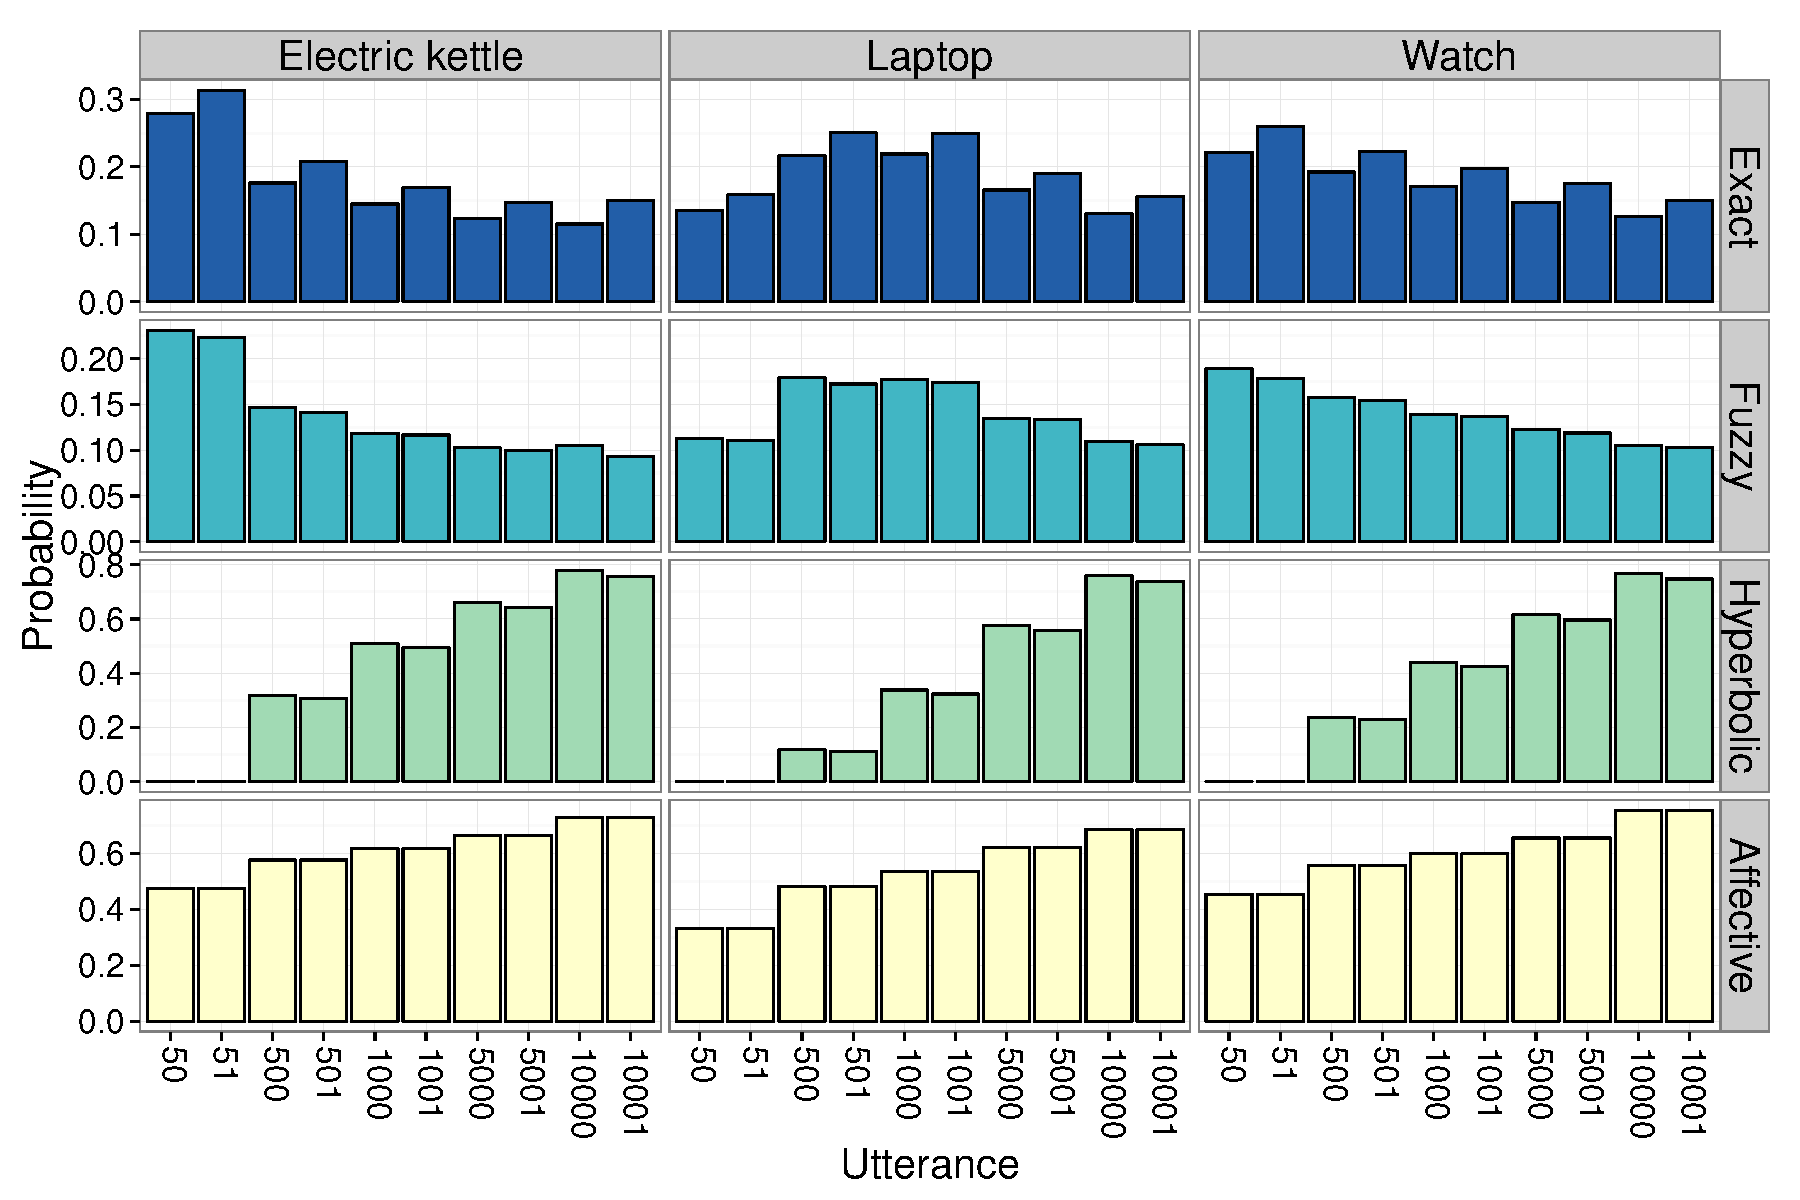
\includegraphics[width=8.7cm]{figure1-revised.pdf}
%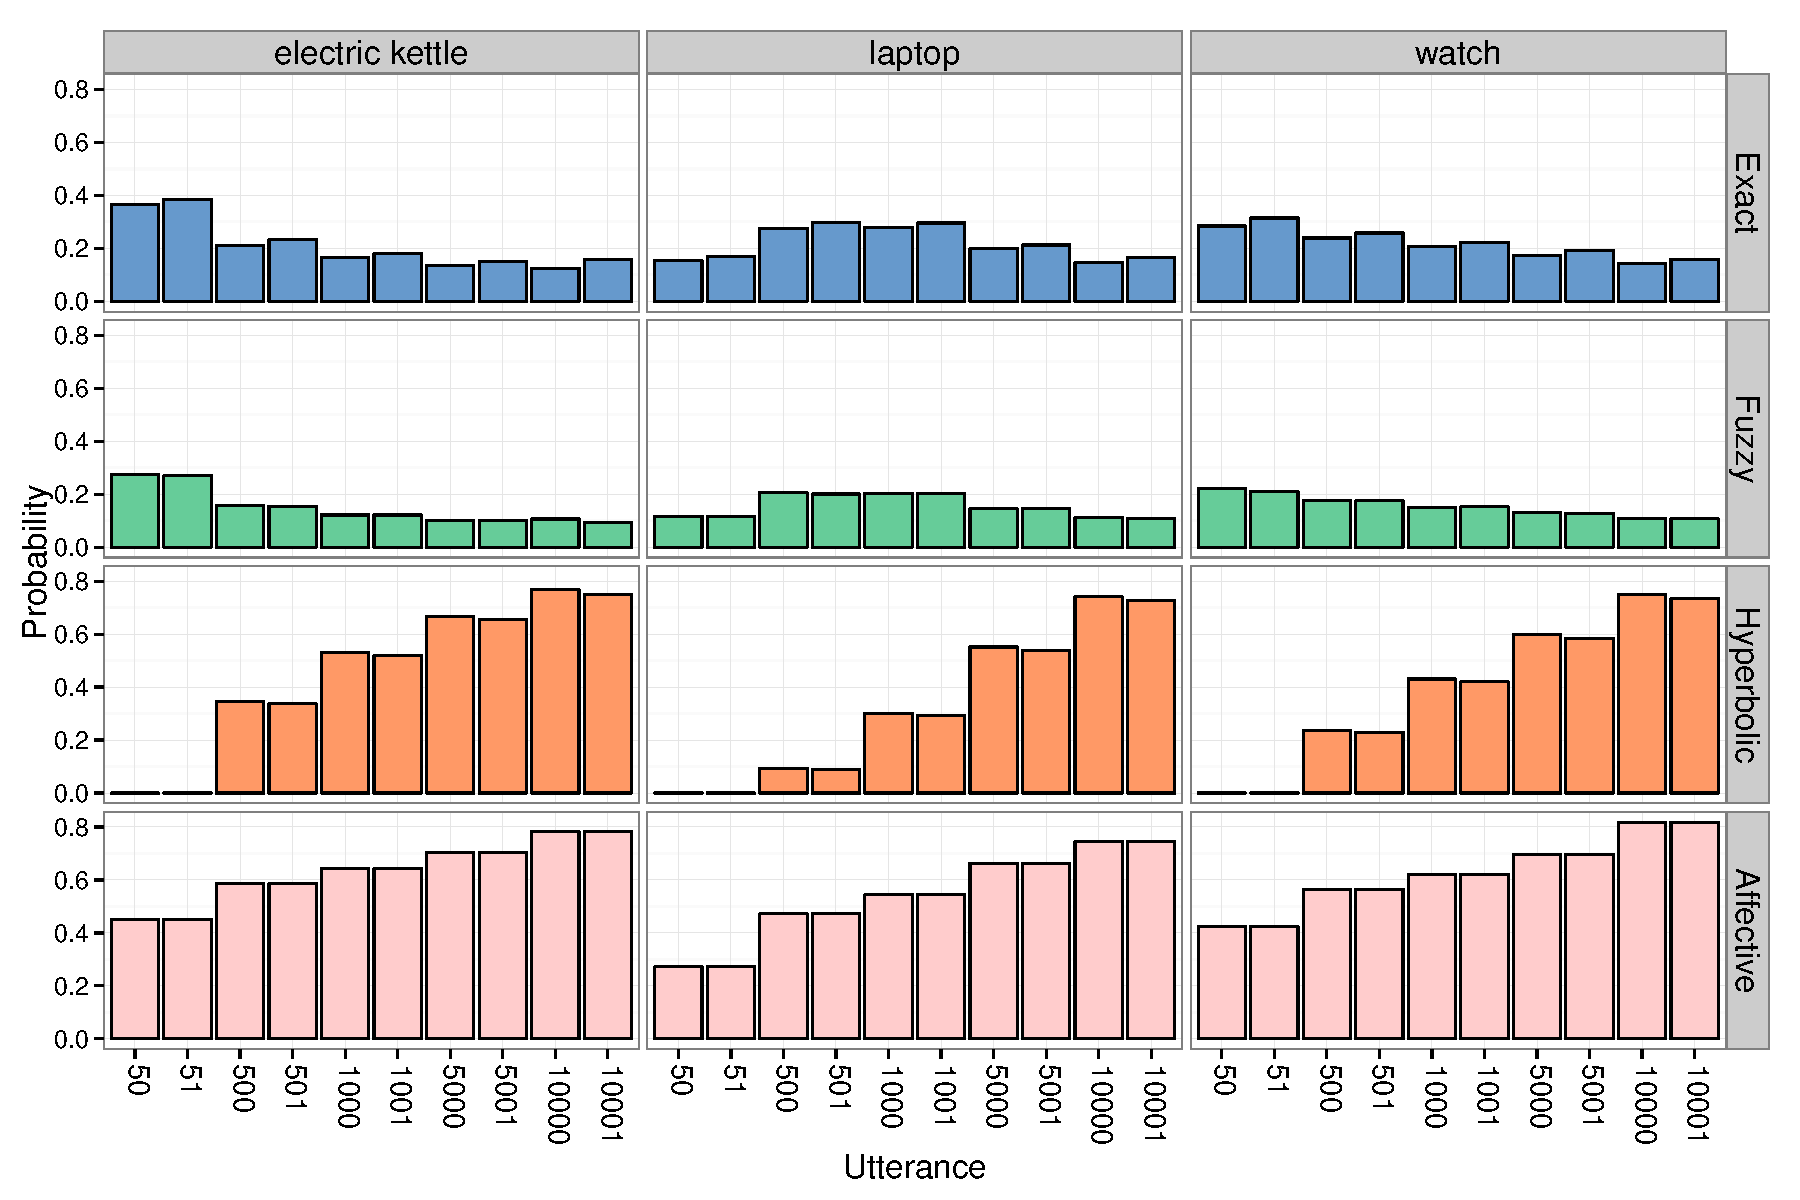
\includegraphics[width=8.7cm]{model_effects.pdf}
\caption{Model predictions of interpretations given utterances. Each bar in the first three rows shows the probability of a type of interpretation given an utterance. Exact interpretations are more likely given sharp rather than round utterances. Fuzzy interpretations are slightly more likely given round utterances. Hyperbolic  interpretations are more likely given more extreme utterances. The final row shows the probability of interpreted affect.} 
\label{model_effects}
\end{minipage}\hfill
\end{figure}

\begin{figure*}
\centering
\begin{minipage}[b]{.49\textwidth}
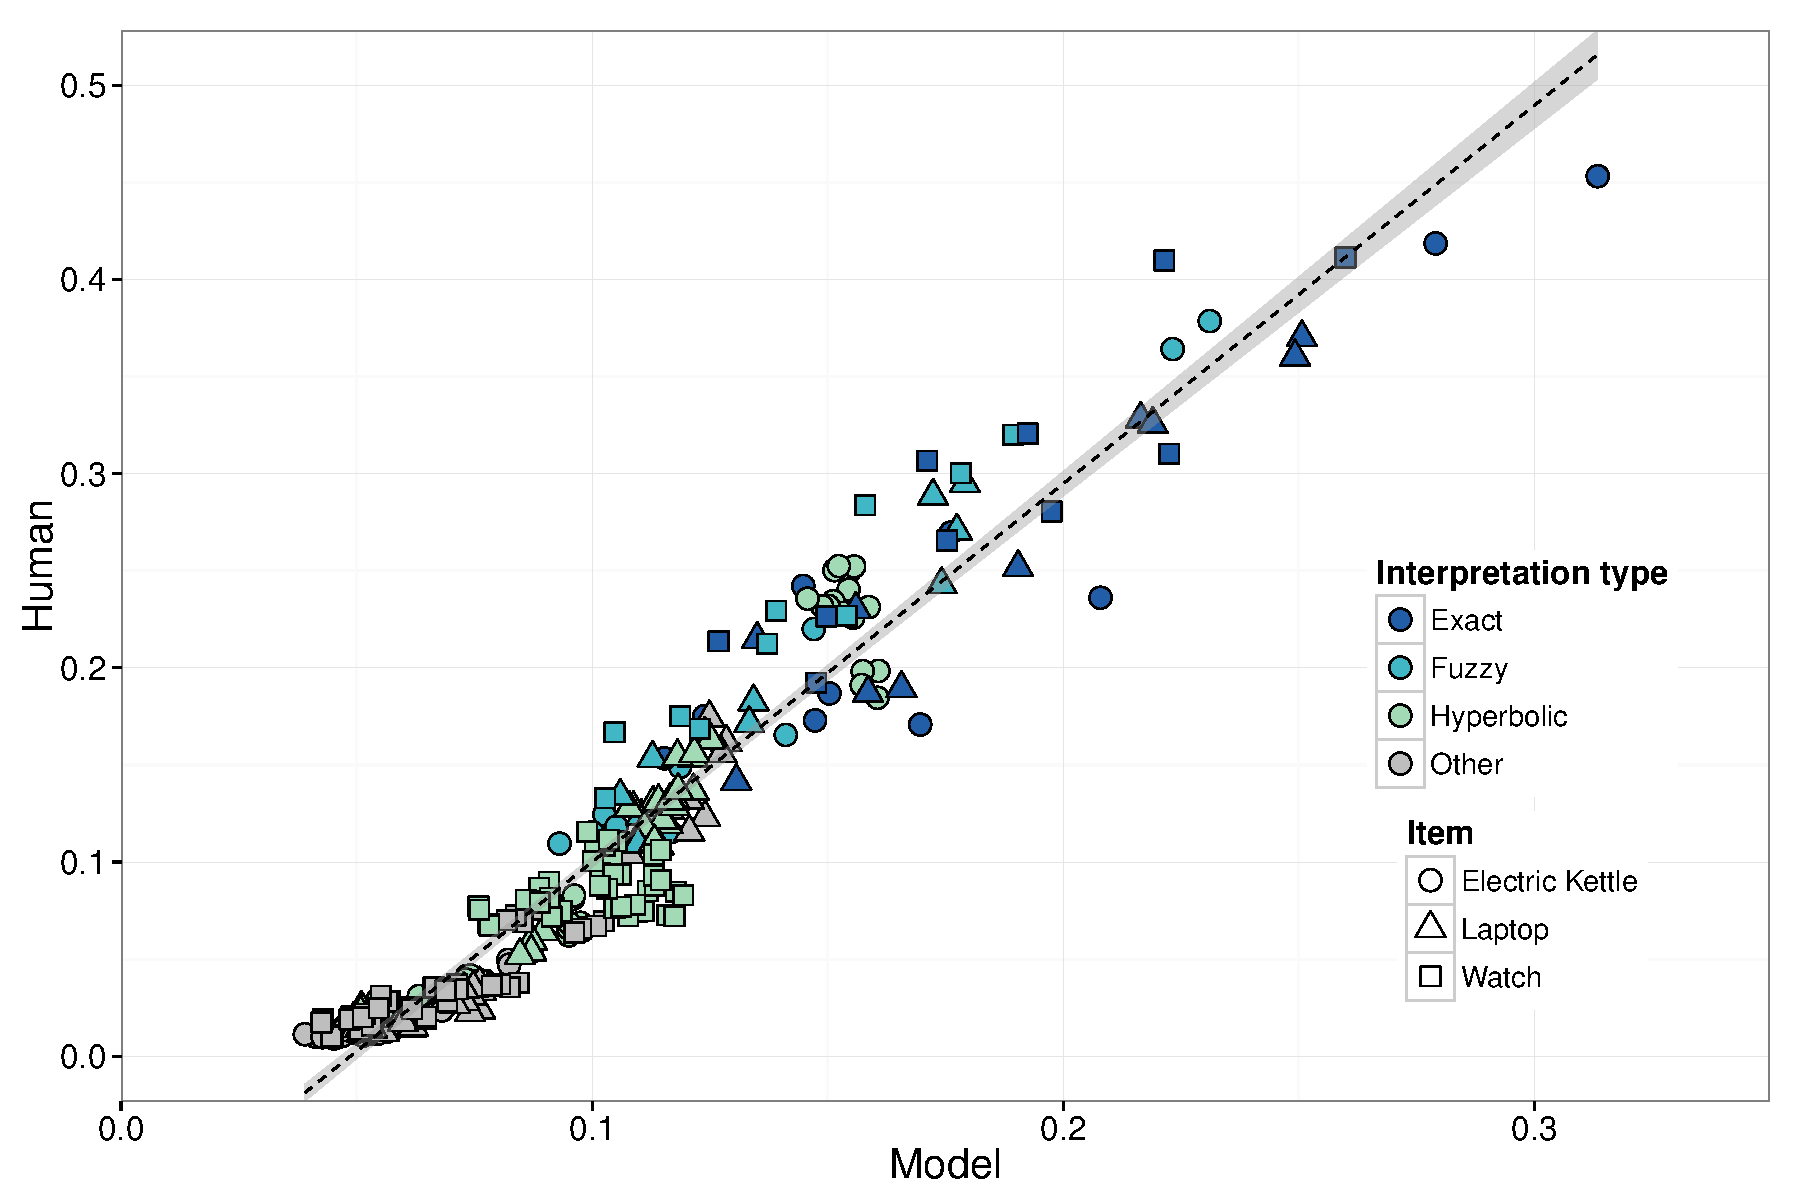
\includegraphics[width=8.7cm]{figure2a-revised.pdf}
\end{minipage}
\begin{minipage}[b]{.49\textwidth}
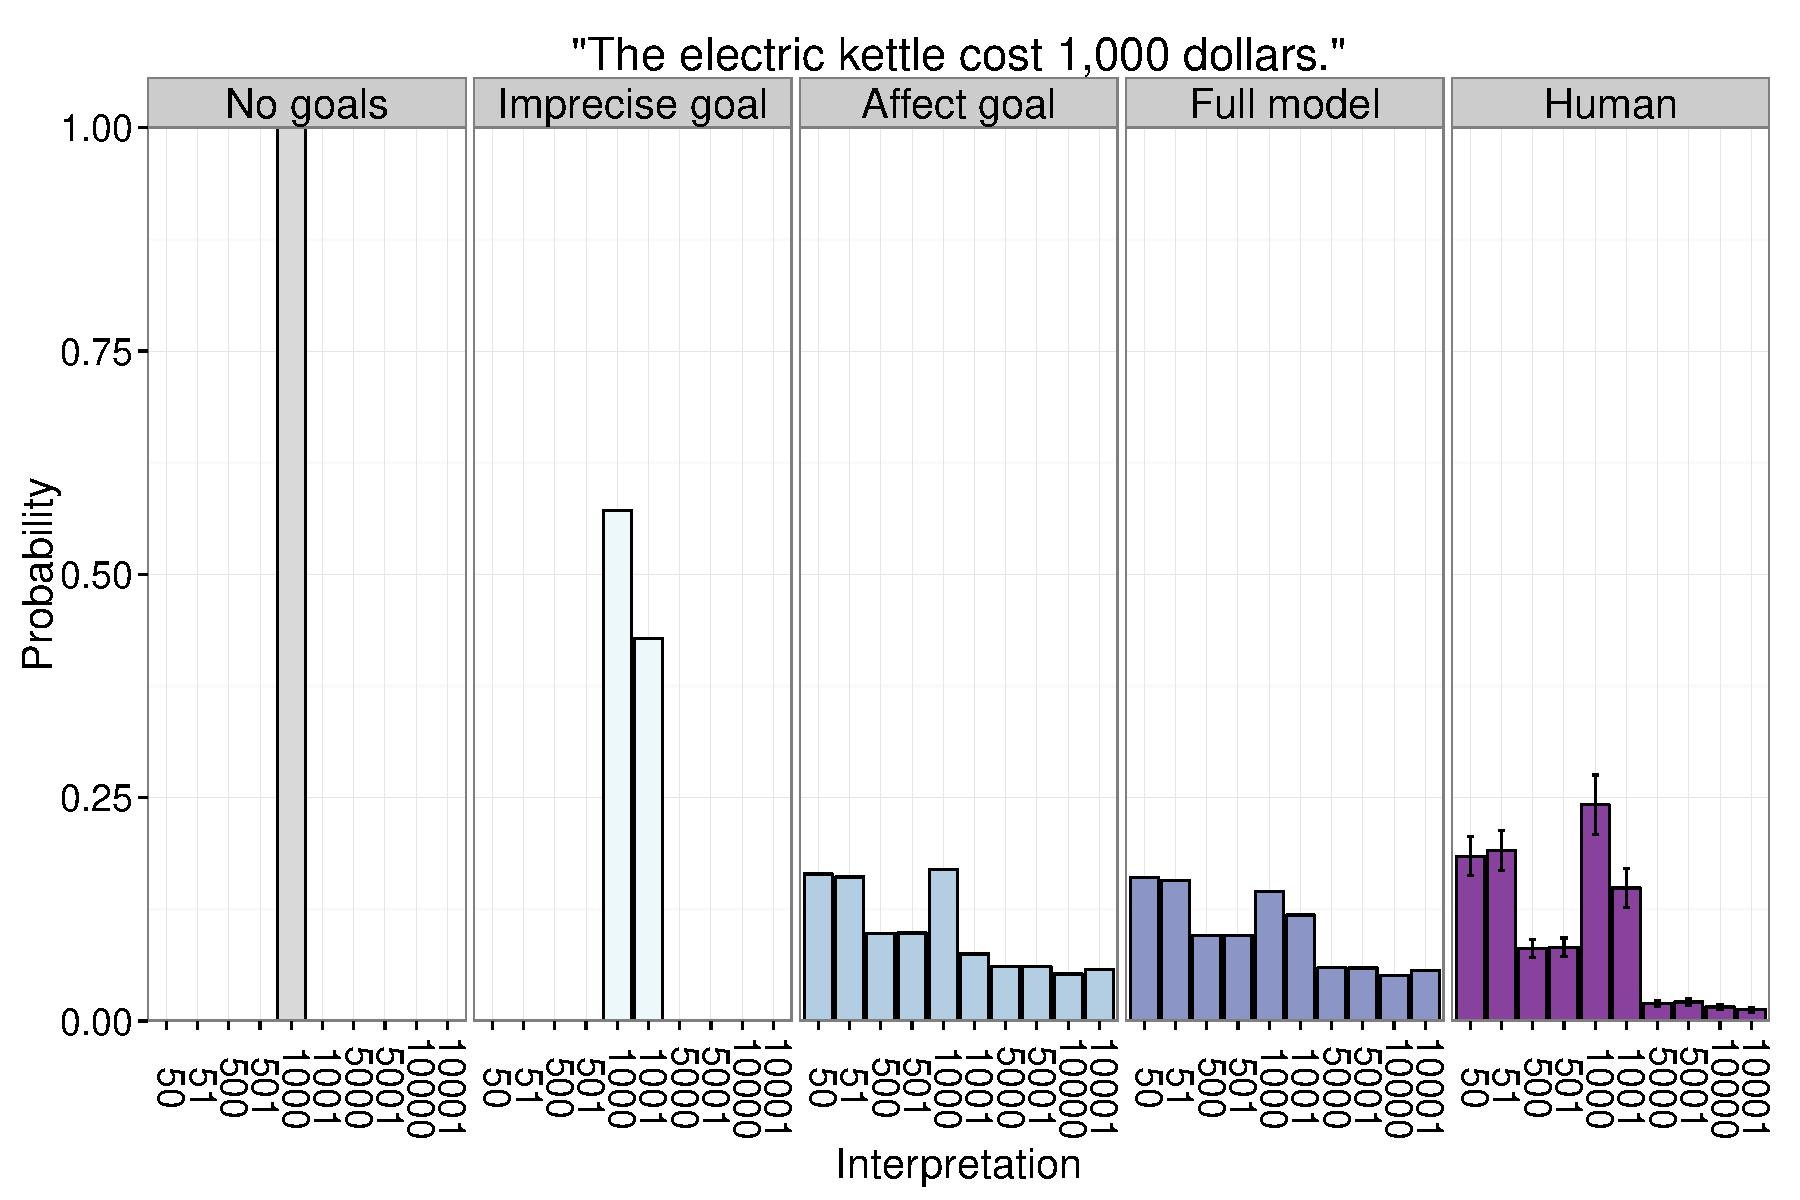
\includegraphics[width=8.7cm]{figure2b-revised.pdf}
\caption{(a) Model predictions v.s. average human responses from Experiment 1. Each point represents an utterance and price state pair ($u, s$). The x-coordinate of each point is the probability of the model interpreting utterance $u$ as meaning price state $s$; the y-coordinate is the empirical probability. Correlation between model and human interpretations is $0.968$ ($95\%$ CI in grey). (b) Comparison of models with different communicative goals and human interpretations for the utterance ``The electric kettle cost 1,000 dollars." A model that considers both affect and precision goals (full model) most closely matches human data.}
\end{minipage}\hfill
\label{model_fit_and_halo}
\end{figure*}

\begin{figure*}

\begin{minipage}[b]{.49\textwidth}
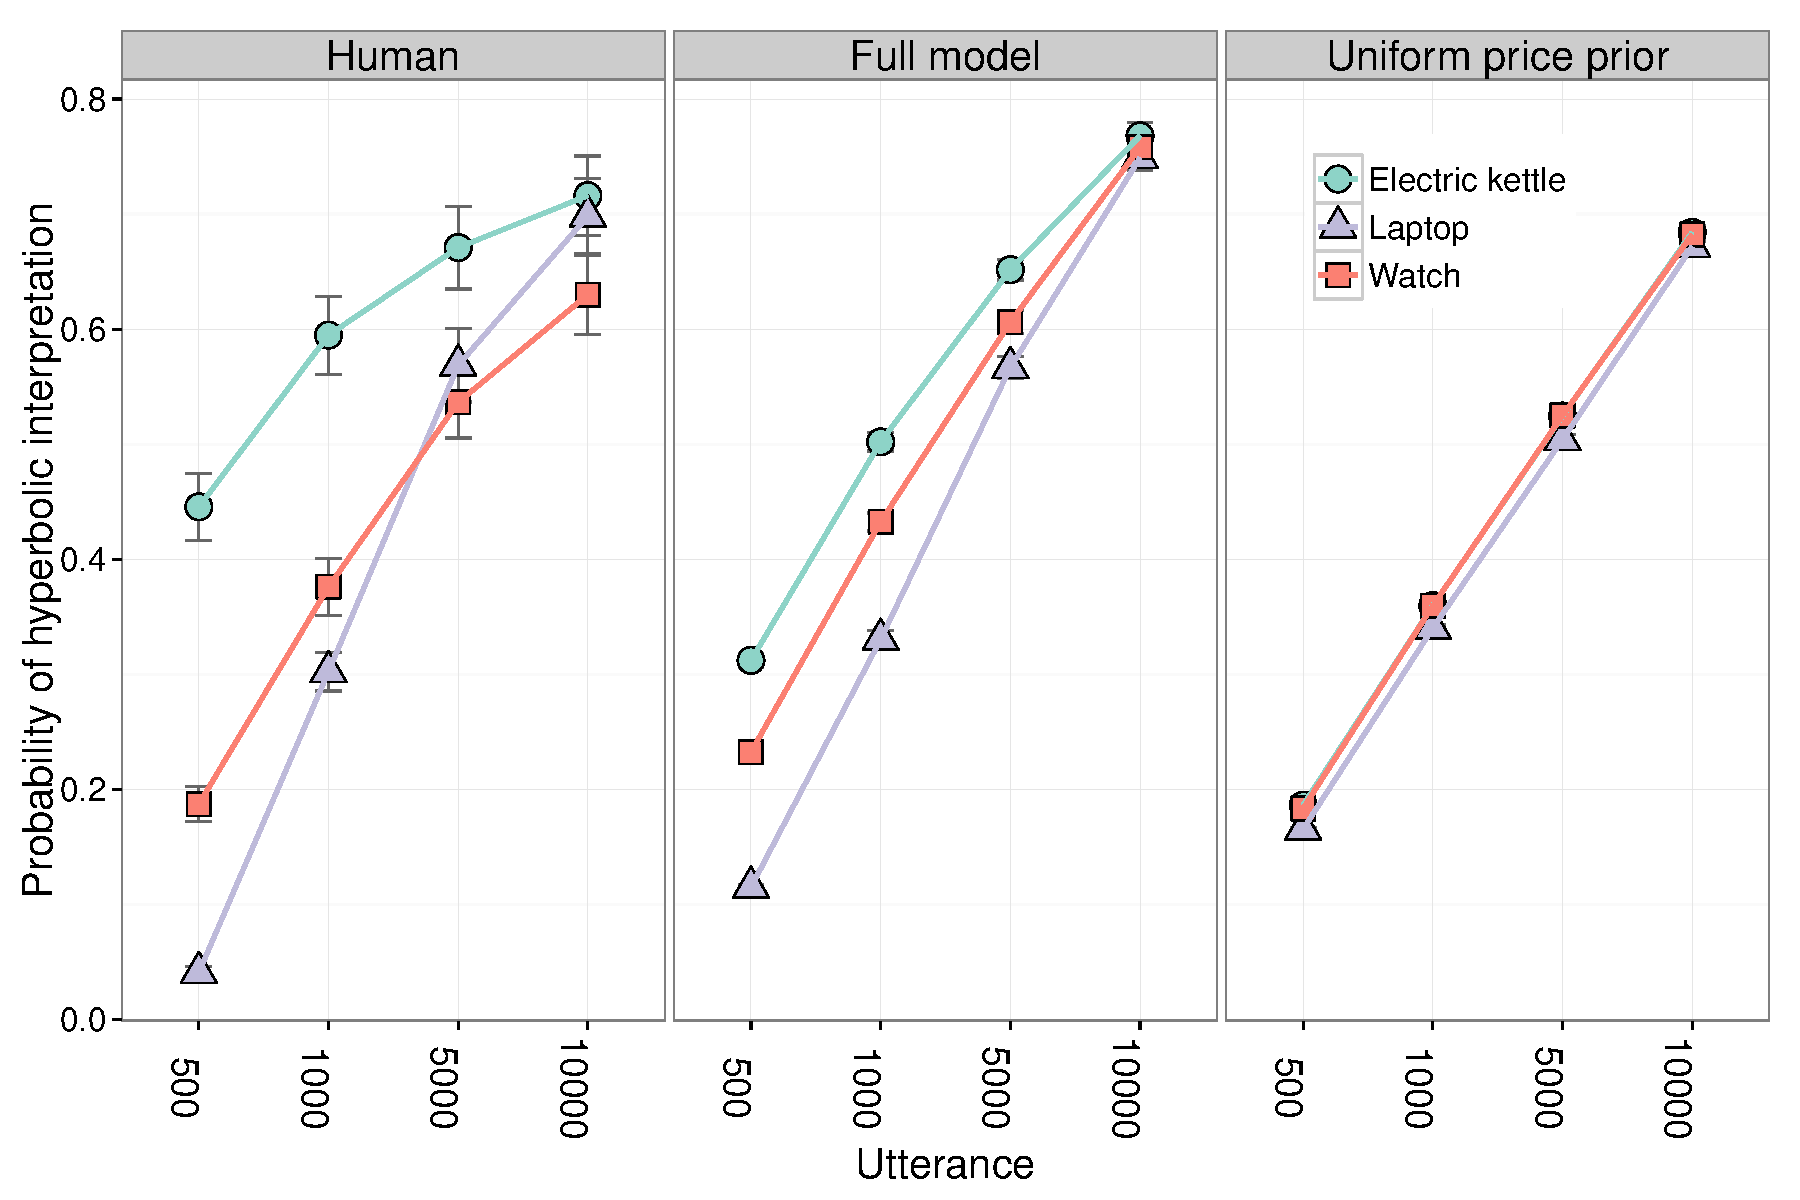
\includegraphics[width=8.7cm]{figure3a-revised.pdf}
\caption{Hello}
\end{minipage}
\begin{minipage}[b]{.49\textwidth}
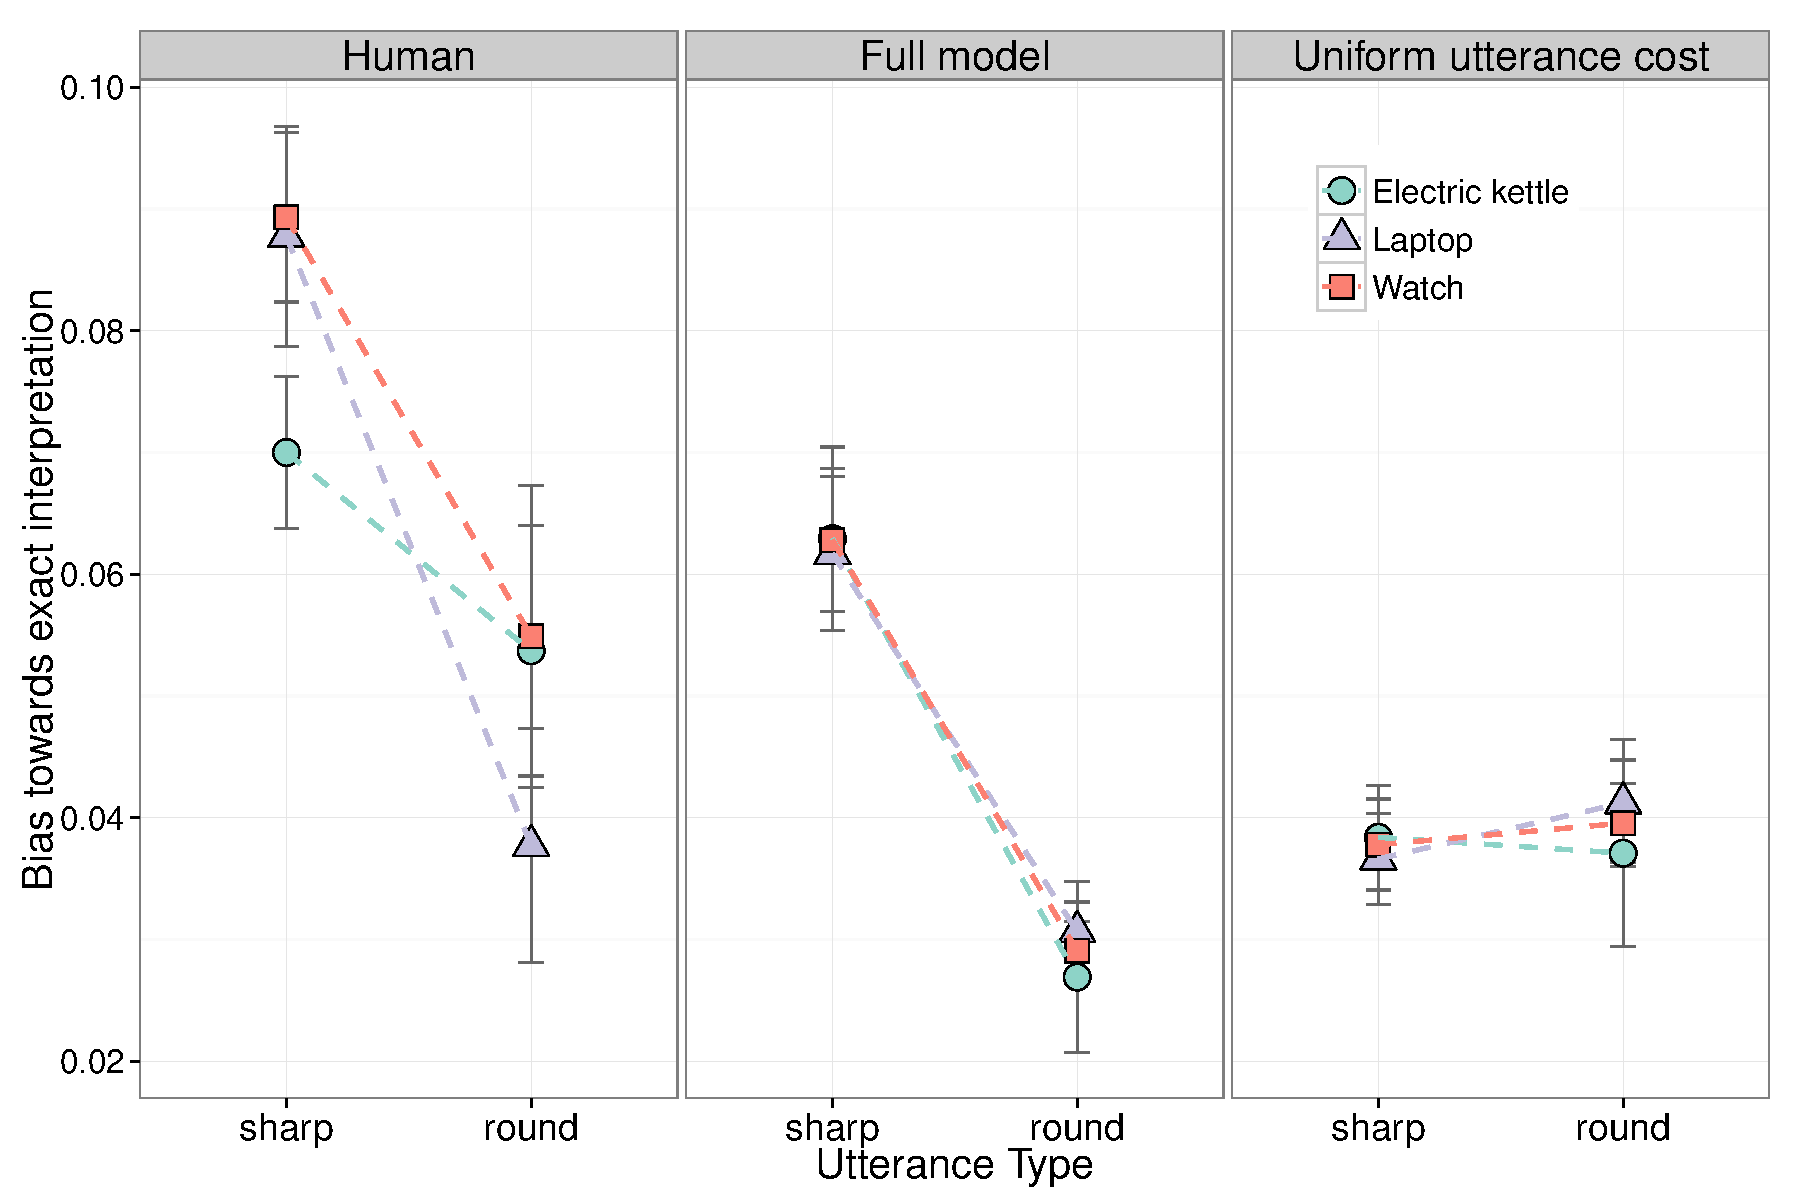
\includegraphics[width=8.7cm]{figure3b-revised.pdf}
\caption{Hello}
\end{minipage}\hfill
\caption{(a) Probability of hyperbolic interpretation given utterances. Leftmost panel shows human data (error bars are standard errors). A full model that uses price priors measured in Experiment 3a demonstrates similar hyperbole effects and distinguishes among item types; a model that uses uniform price priors does not. (b) Halo effect as measure by bias towards exact interpretation for round/sharp utterance types. Humans' bias towards exact interpretation is significantly higher for sharp numbers. A full model that assigns higher cost to sharp numbers captures this result; a model that uses uniform utterance cost does not.}
\label{hyperbole_and_affect}
\end{figure*}


\subsection{Model simulations}

Using the price priors and affect priors measured for each of the three items, we obtained the meaning distributions predicted by the model for all utterances (see Figure \ref{full_bar}a). Figure 1 summarizes this distribution into different types of interpretations. The first three are model interpretations regarding the price state: exact (e.g.,  ``1000" interpreted as $1000$), fuzzy (e.g. ``1000" interpreted as 1001), and hyperbolic (e.g. ``1000" interpreted as 100). Round utterances such as ``500" and ``1000" are interpreted less exactly and more fuzzily than their sharp counterparts, which captures pragmatic halo. Utterances whose literal meanings are less likely given the price prior are more likely to be interpreted hyperbolically (e.g. ``1000" is more likely to be interpreted hyperbolically for electric kettles than laptops), which captures a basic feature of hyperbole. Affective interpretation refers to the probability that an utterance conveys the speaker's opinion that the price is expensive. Utterances whose literal meanings are associated with higher affect priors (such as ``10000" and ``10001") are more likely to be interpreted as conveying affect, which predicts the affective subtext of hyperbole. 

To build intuition for these predictions, consider a pragmatic listener who reasons about a speaker and analyzes her choice of utterance. The pragmatic listener hears ``10,000 dollars" and knows that its literal meaning is extremely unlikely. Given that the speaker reasons about a literal listener who interprets ``10,000 dollars" literally and believes that the speaker very likely thinks it is expensive, ``10,000 dollars" is an  informative utterance if the speaker's goal is to communicate an opinion that the kettle is expensive (without concern for the actual price). Since the pragmatic listener uses this information to perform joint inference on the speaker's communicative goal and the meaning of the utterance, he infers that ``10,000 dollars" is likely to mean less than 10,000 dollars but that the speaker thinks it is too expensive.
 

\subsection{Behavioral experiments}

We conducted Experiment 1 to evaluate the model's predictions for the interpreted price. Participants read scenarios in which a buyer produces an utterance about the price of an item he bought, for example: ``The electric kettle cost 1000 dollars." Participants then rate the likelihood that the item cost $s$ dollars for $s \in S$ (see Experiment 1). Figure \ref{full_bar}b shows humans' interpretation distributions across all utterances.  Participants were more likely to interpret utterances as hyperbolic when their literal meanings have lower probabilities under the item's prior price distribution ($F(1, 10) = 44.06, p < 0.0001$). To examine the halo effect, we computed the difference between the probability of an exact interpretation and the probability of a fuzzy interpretation for each utterance. This difference is significantly smaller for round numbers than for sharp numbers ($F(1, 28)=18.94,  p < 0.001$), which indicates that round numbers tend to be interpreted less precisely than sharp numbers. To quantitatively evaluate the model's fit, we compared model and human interpretation probabilities across all utterances and showed that model predictions are highly correlated with human interpretations of number words ($r=0.968, p<0.0001$) (Figure \ref{model_fit_and_halo}a; see Materials and Methods for details). 

To show how each component of the proposed model is necessary to capture effects observed in the human data, we explore a series of simpler comparison models. For illustration, Figure \ref{model_fit_and_halo}b compares model interpretations of the utterance ``The electric kettle cost 1,000 dollars" given inference over different communicative goals. A model that does not consider alternative goals interprets the utterance entirely literally. Note that even though such a model has information about the affect dimension (i.e. $P_A$), without goal inference it is unable to produce nonliteral interpretations because it assumes that the speaker only wants to maximize informativeness along the same dimension as the utterance, i.e. the price state. A model that considers a speaker whose goal may be to communicate precisely or imprecisely interprets the utterance as meaning either 1000 or 1001. A model that considers a speaker whose goal may be to communicate the price state \emph{or} her affect prefers price states with higher prior probabilities. Finally, a model that considers the full range of goals demonstrates hyperbole and halo effects that closely match humans' interpretations. To demonstrate that our model is able to usefully incorporate nonlinguistic knowledge to infer the meaning of utterances, Figure \ref{hyperbole_and_affect}a shows the hyperbole effect as measured by the probability that an utterance $u$ is interpreted as price state $s$ such that $u > s$. A full model that uses empirically measured price priors captures humans' interpretations, while a model that takes a uniform distribution over price states does not. To demonstrate that our model is able to utilize utterance costs and goal inference to capture pragmatic halo, Figure \ref{hyperbole_and_affect}b shows the halo effect as measured by the bias towards exact interpretation for sharp versus round numbers. A full model that assigns higher utterance costs to sharp numbers captures the significant difference in humans' biases for sharp versus round numbers, while a model where utterance costs are uniform does not. These analyses suggest that extending the RSA framework to include goal inference, incorporating empirically measured background knowledge, and including information about utterance costs all contribute to the model's ability to understand nonliteral language.
\begin{figure*}
\centering
\begin{minipage}[b]{.49\textwidth}
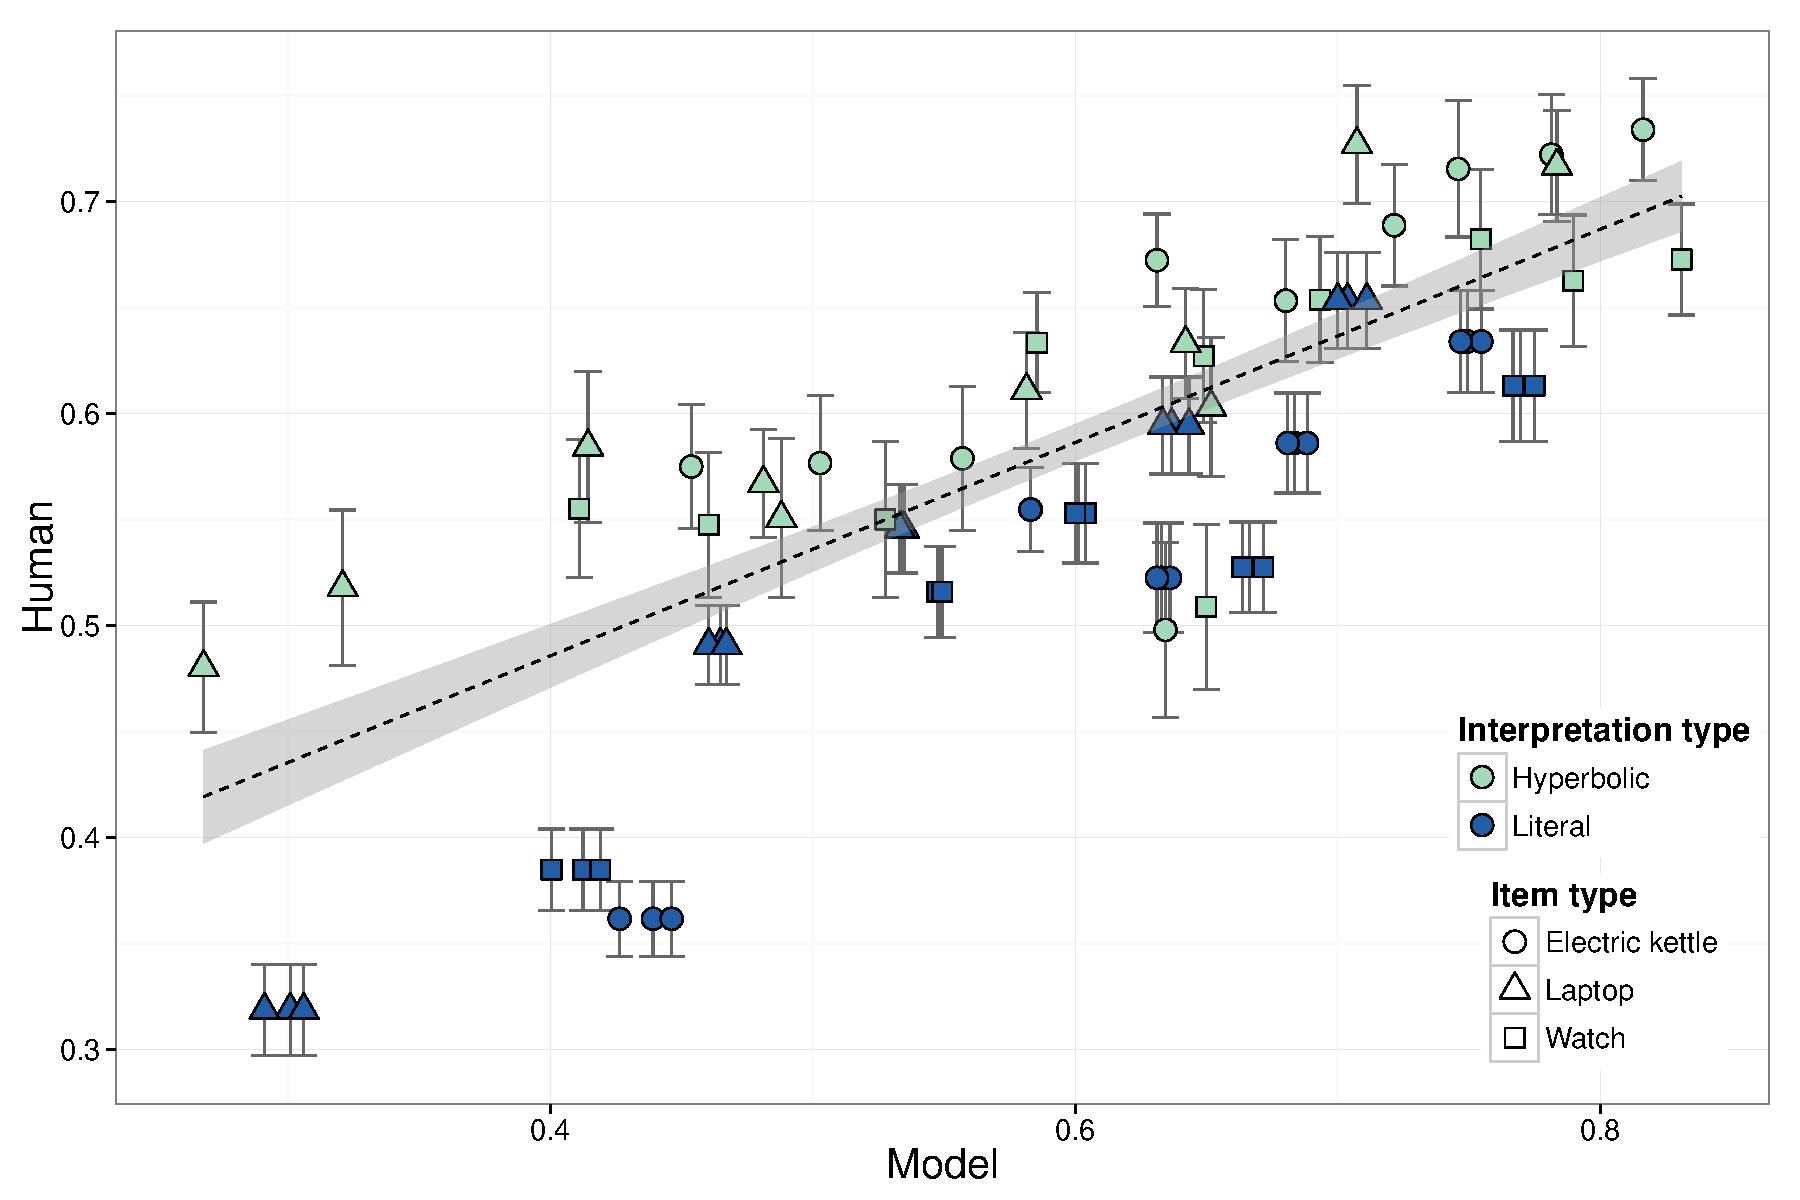
\includegraphics[width=8.7cm]{figure4a-revised.pdf}
\caption{Hello}
\end{minipage}
\begin{minipage}[b]{.49\textwidth}
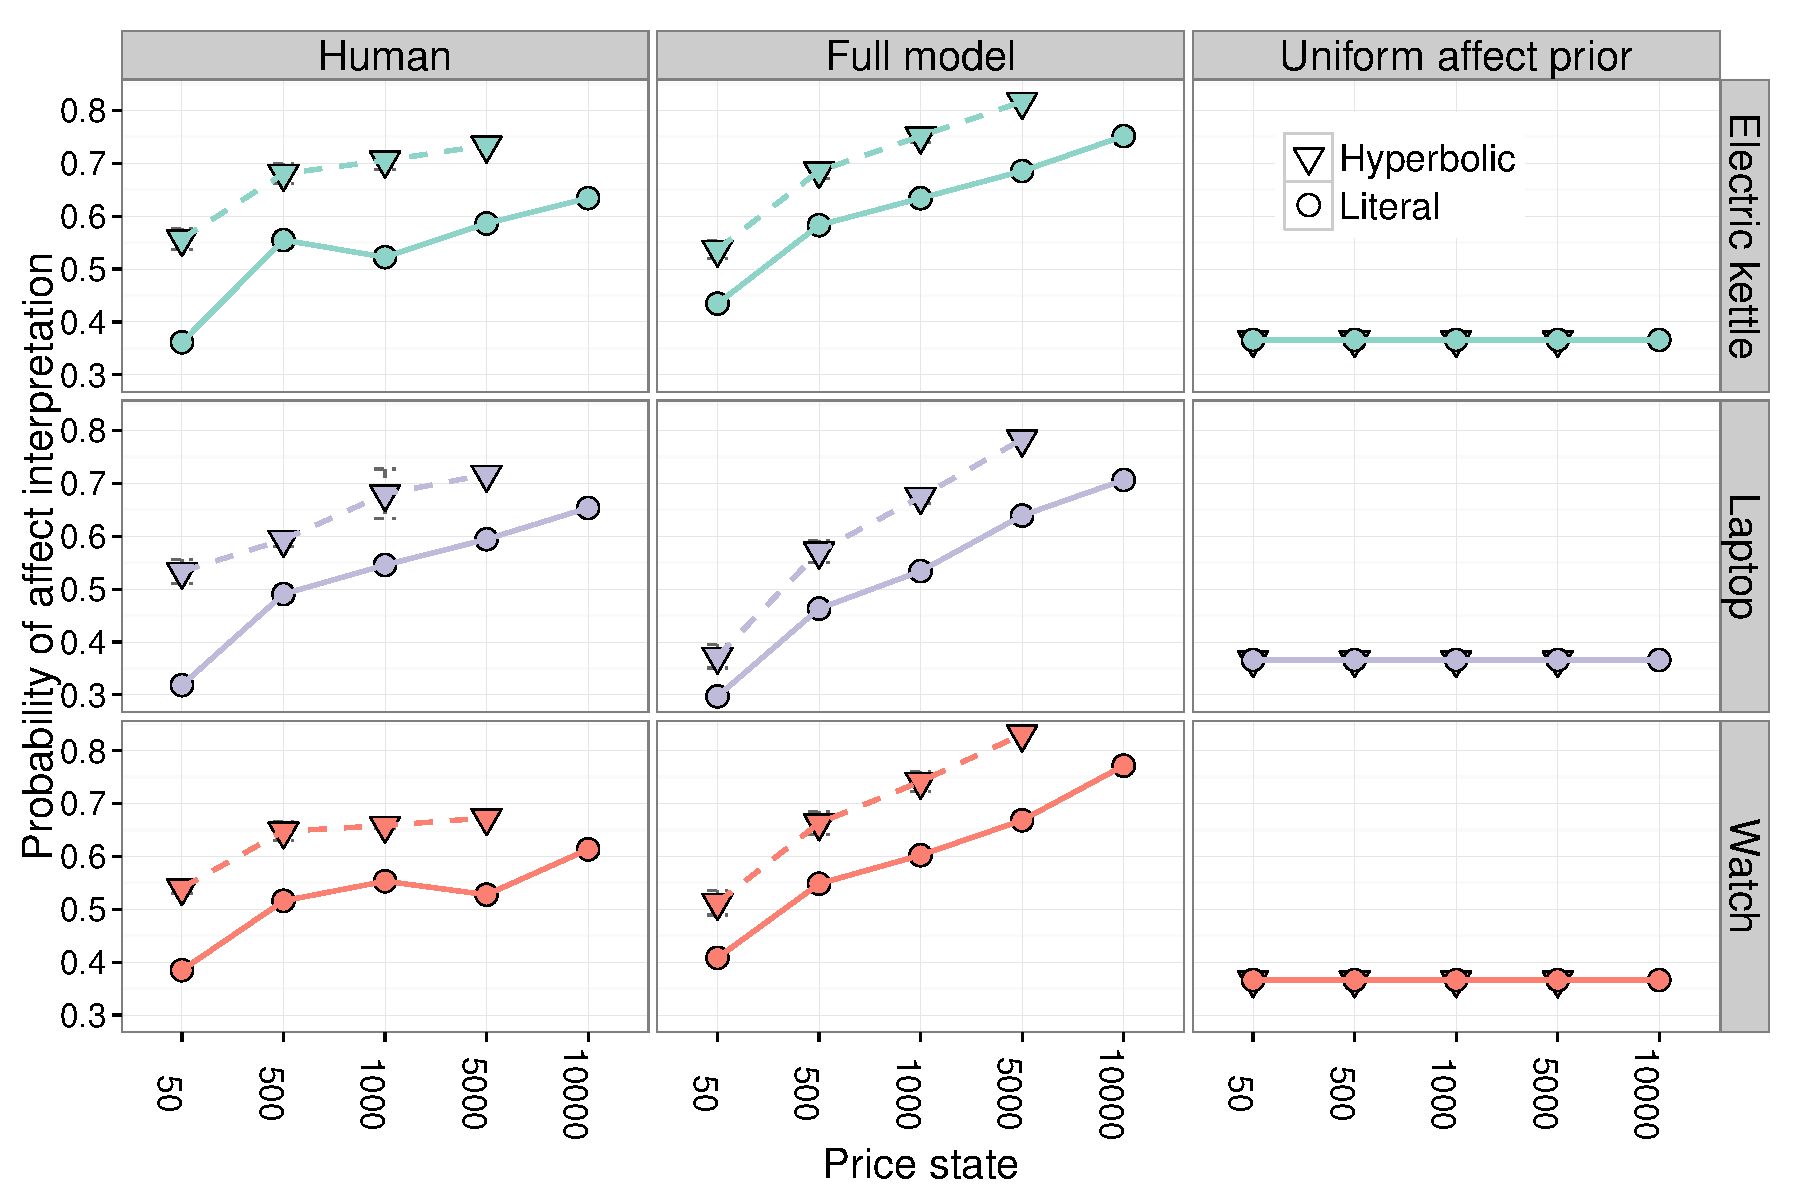
\includegraphics[width=8.7cm]{figure4b-revised.pdf}
\caption{Hello}
\end{minipage}
\caption{(a) Model predictions of affect v.s. human responses from Experiment 2. Each point represents an utterance and price state pair $(u, s)$. For pairs where $u = s$, the utterance is literal (blue); for $u > s$, the utterance is hyperbolic (green). The x-coordinate of each point is the model's prediction of the probability that the utterance/price state pair conveys affect; the y-coordinate is participants' ratings (error bars are standard error). Correlation between model and humans is $0.775$ ($95\%$ CI in grey). (b) Probability of interpreting a hyperbolic/literal utterance as conveying affect. For the same price state, humans infer higher probability of affect given hyperbolic utterances (triangle) than literal (round). A model that uses affect priors measured in Experiment 3b captures this result; a model that uses uniform affect priors does not.}
\label{affect_exp}
\end{figure*}

Does the model capture the rhetorical effect of hyperbole? We conducted Experiment 2 to examine humans' interpretation of affect in hyperbolic versus literal utterances. Participants read scenarios in which a speaker bought an item that cost $s$ dollars and says it cost $u$ dollars, where $u \geq s$. They then rate how likely it is that the buyer thinks the item was too expensive (see Experiment 2). We focused on the affect of an item being too expensive because previous findings suggest that hyperbole is more often used to communicate negative rather than positive attitudes \cite{roberts1994, mccarthy2004there}. Results showed that utterances $u$ where $u > s$ are rated as significantly more likely to convey affect than utterances where $u {=} s$ ($F(1, 25)=12.57, p < 0.005$). This suggests that listeners infer affect from hyperbolic utterances above and beyond the affect associated a priori with a given price state. Quantitatively, we compared model and human interpretations of affect for each of the 45 utterance and pice state pairs $(u, s)$ where $u \geq s$. While there is a significant amount of noise in the human judgments (average split-half correlation is $0.833$), the model predicts human interpretations of the utterances' affective subtext significantly better than chance ($r=0.775, p < 0.00001$), capturing most of the reliable variation in these data (Figure \ref{affect_exp}a). To demonstrate how our model explains this effect, Figure \ref{affect_exp}b shows probabilities of affect given a price state and a literal or hyperbolic utterance. The human data shows that higher actual price states are associated with higher probabilities of affect. Within the same price state, hyperbolic utterances are interpreted as conveying more affect than literal utterances. These effects are replicated by the full model, but not by a model that takes in a uniform affect prior. This analysis suggests that the rhetorical effect of hyperbole is driven in part by people's shared knowledge about prices and associated affect. 

\section{Discussion}
We presented the first computational model of nonliteral understanding that quantitatively predicts people's hyperbolic and imprecise interpretations of number words.  
Our behavioral results show that complex patterns in number interpretation depend on common knowledge between speaker and listener, consideration of communicative efficiency, and, critically, reasoning about the speaker's communicative goal.
Our model represents an explicit, computational-level hypothesis about how these factors are integrated to give rise to the particular, graded interpretations that people arrive at. 
The model's quantitative predictions closely match humans' judgments, including cases of hyperbole, a complex phenomenon previously beyond the scope of computational models.
%The model is intended to give a computational-level account of how people utilize prior knowledge and pragmatic reasoning to arrive at nonliteral interpretations of language. 
%
%It is mute on process-level details, such as whether literal interpretations must be considered before they are rejected in favor of nonliteral interpretations. Instead, our goal was to show that formalizations of basic communicative principles---informativity with respect to a goal---can explain nonliteral language understanding as well as its rhetorical effects. 
%
%We were able to examine usage of number words at a fine-grained level and understand in quantitative detail
%how the details of an utterance in context predict specific interpretations of a number word. 
%how various factors---background knowledge, literal meaning, affective dimensions, topic---are integrated together in language understanding to give rise to the particular, graded interpretations that people arrive at. 
%Our model's predictions closely match humans' judgments of hyperbole, a complex phenomenon previously beyond the scope of computational models.

The current approach has important connections to theories of communication and linguistic meaning. 
Our speaker aims to be informative, as in Gricean theories of communication, but only with respect to a particular goal or topic---realizing a kind of relevance principle. This relevance is critical for deriving non-literal interpretations in our model.
%By modeling the speaker as choosing an utterance that maximizes informativeness with respect to her goal, we showed that people can infer nonliteral meaning by assuming that the speaker follows a principle of relevance. 
%By introducing a dimension of meaning that is associated with a state of the world and not encoded into the semantics of an utterance, we formalized an encyclopedic approach to meaning that views meaning as a combination of linguistic and extralinguistic knowledge. 
While our model is currently limited to two dimensions of meaning and corresponding goals, in future work we hope to capture dimensions central to other figures of speech such as irony and metaphor, thus extending our model to explain nonliteral language more broadly. We believe that our framework significantly advances the flexibility and richness of formal models of language understanding, such that some day probabilistic models will explain \emph{everything} (hyperbolically speaking). 

%----------------------------------------------------------------------------------------
%	MATERIALS AND METHODS
%----------------------------------------------------------------------------------------

%% Optional Materials and Methods Section
%% The Materials and Methods section header will be added automatically.

\begin{materials}
\begin{figure*}[tbh]
\label{full_bar}
\centering
\begin{minipage}[b]{.495\textwidth}
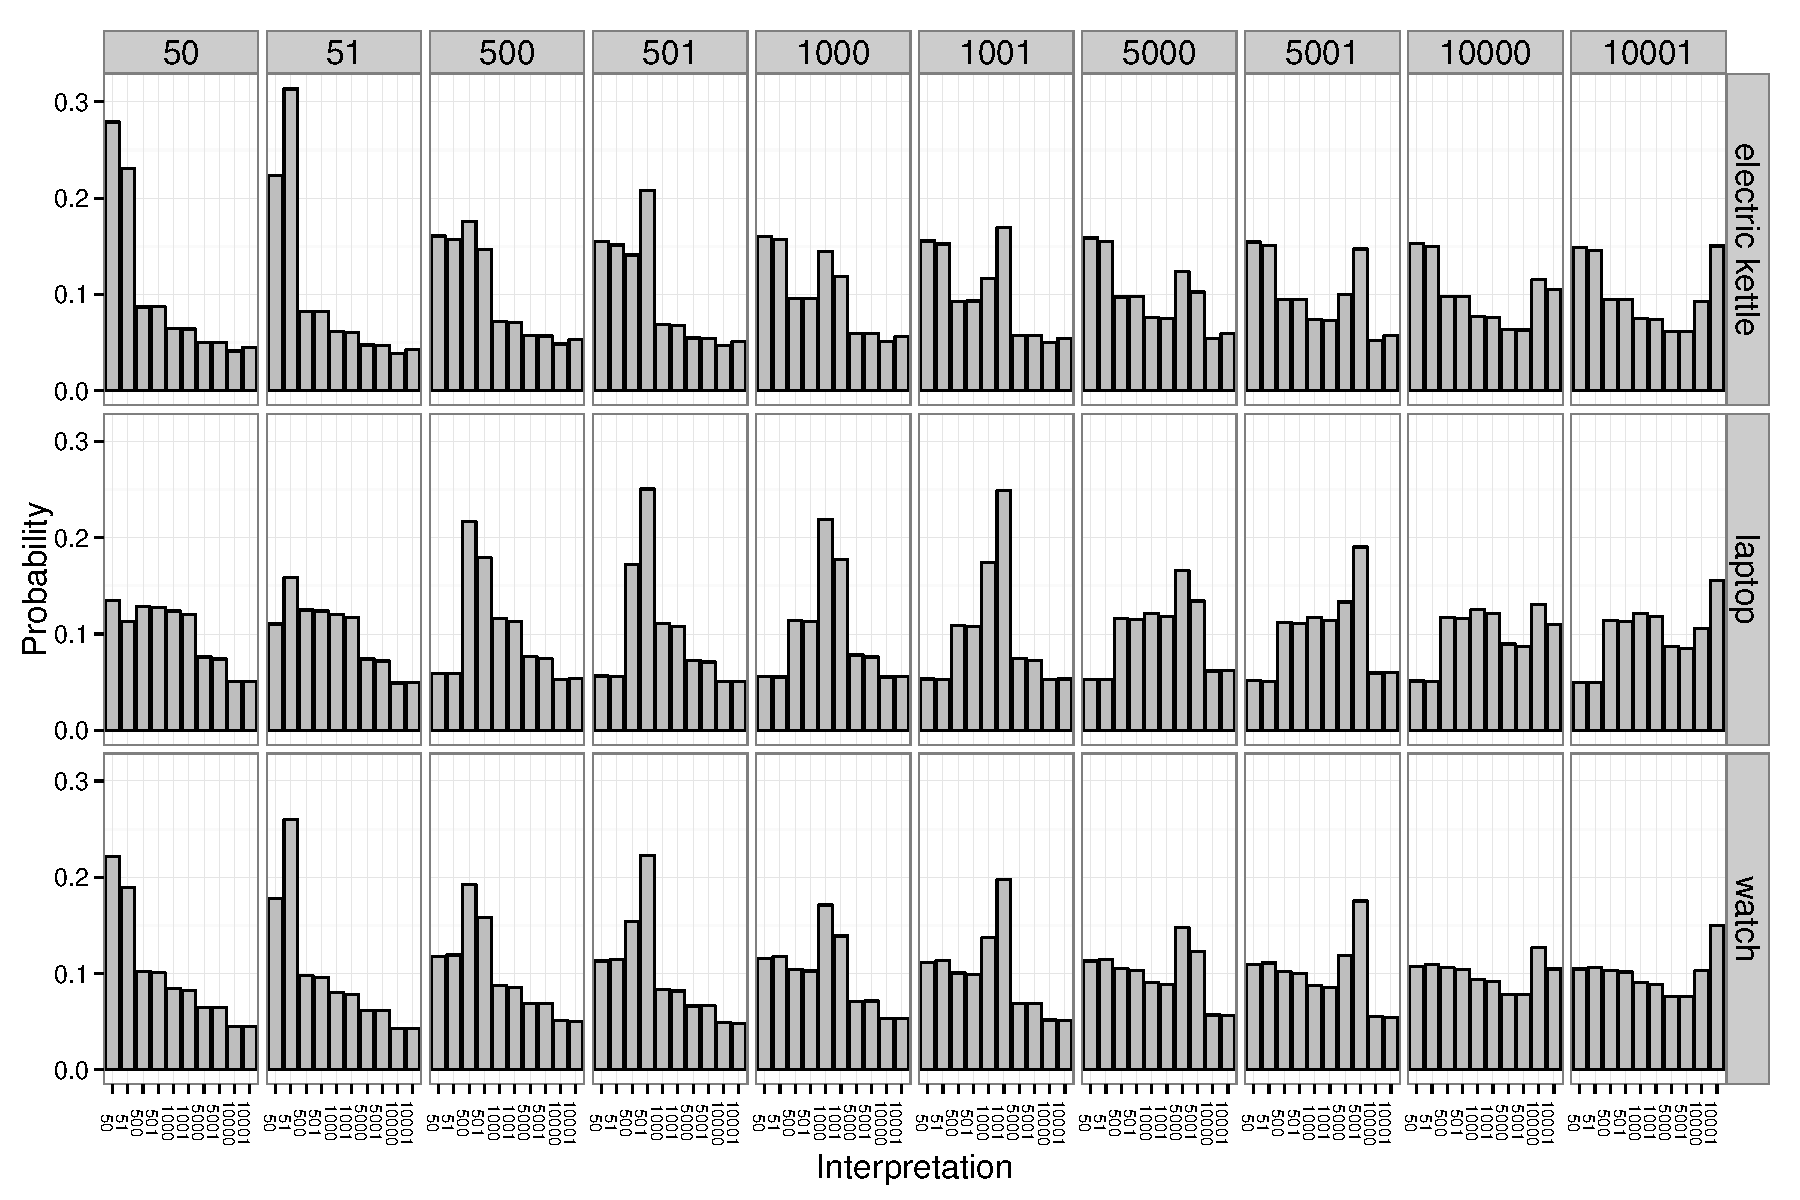
\includegraphics[width=9cm]{figure5a-revised.pdf}
\end{minipage}
\begin{minipage}[b]{.495\textwidth}
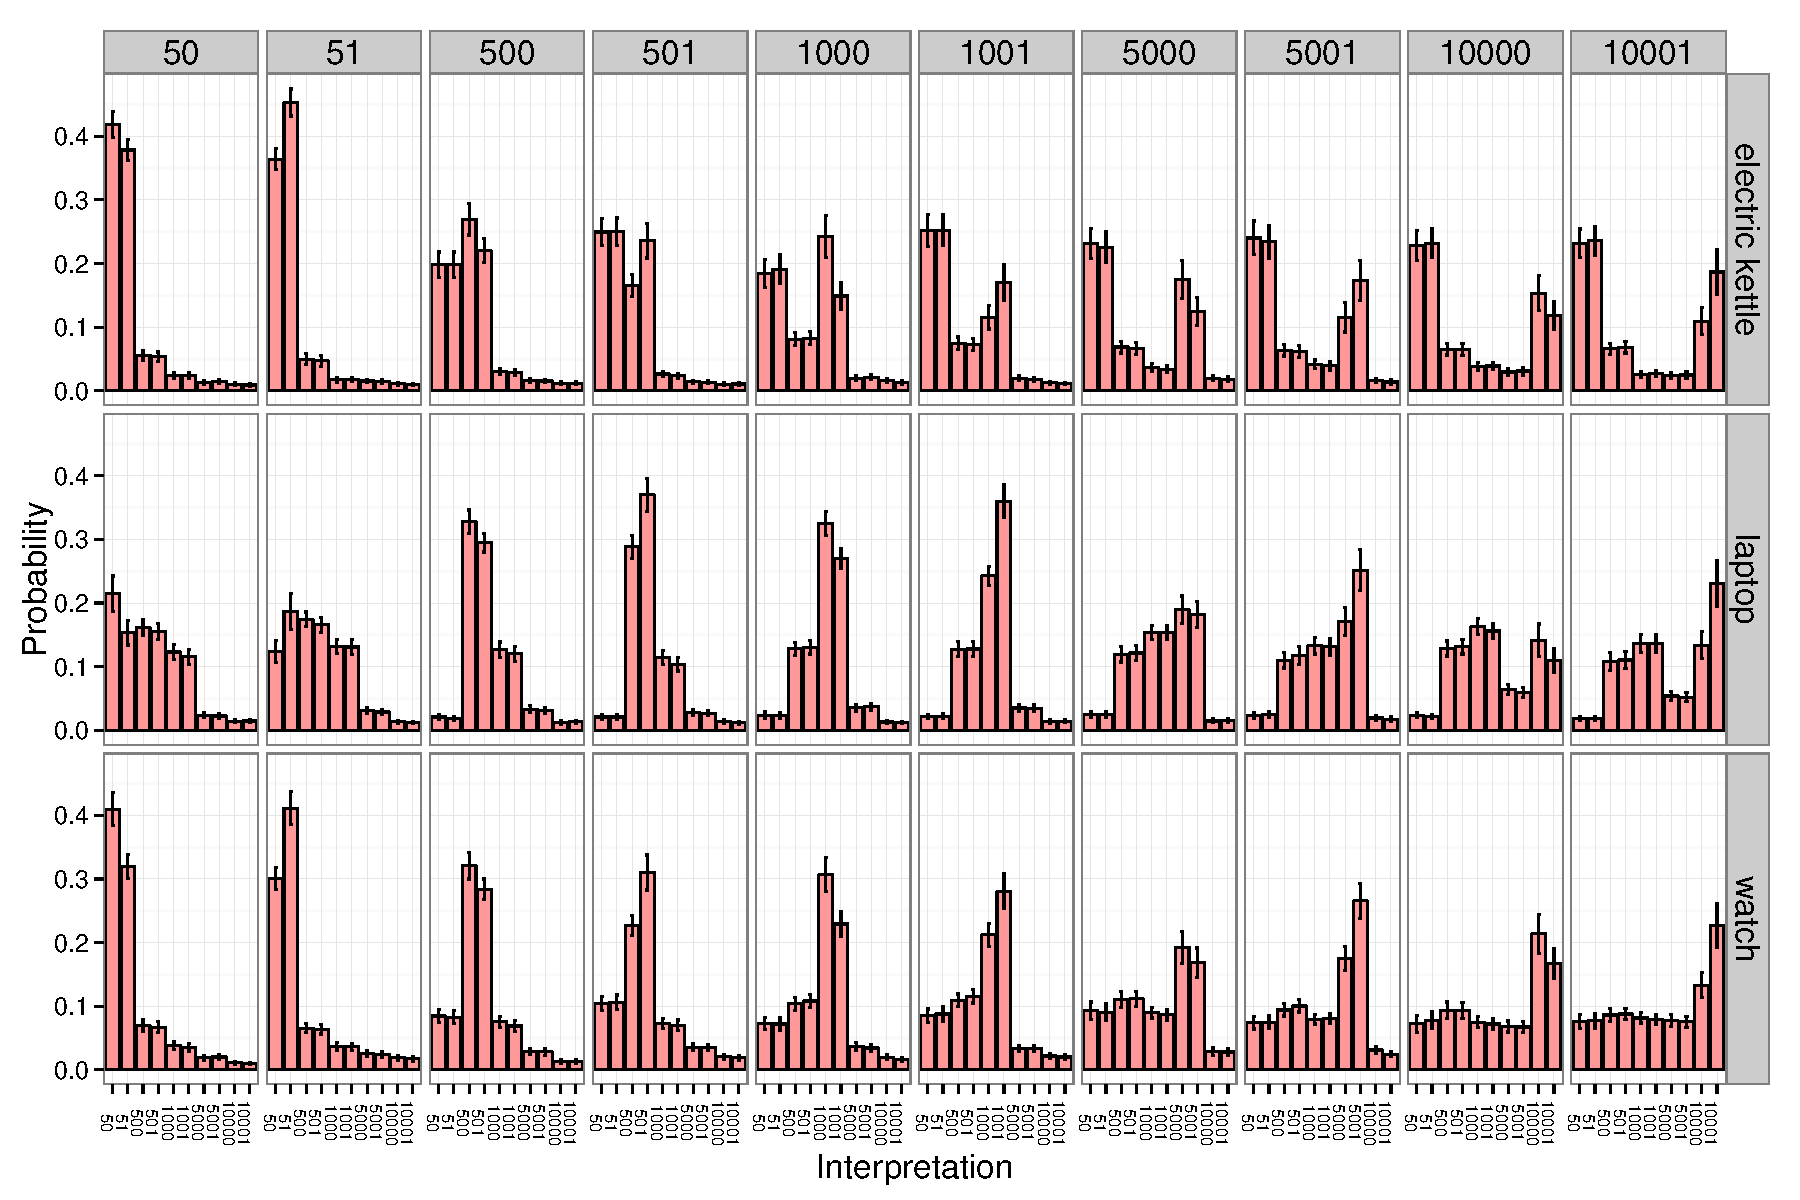
\includegraphics[width=9cm]{figure5b-revised.pdf}
\end{minipage}
\caption{(a) Posterior price state distributions predicted by the model given utterances. Each panel shows the interpretation distribution of an utterance. (b) Price state distributions rated by participants given utterances. Each panel shows the interpretation distribution of an utterance. Error bars are standard errors.}
\end{figure*}
\section{Model}
Let $u$ be an utterance. The meaning of $u$ has two dimensions: the actual price state $s$ and the speaker's affect $a$. We defined the set of price states $S=\{50, 51, 500, 501, 1000, 1001, 5000, 5001, 10000, 10001\}$. We assumed that the set of utterances $U$ is identical to $S$. We defined the set of affect states $A=\{0, 1\}$ (0 means no affect and 1 means with affect---this binarization is purely for simplicity). Given $S$ and $A$, the set of possible meanings $M$ is given by $M = S \times A$. We denote each meaning as $s, a$, where $s \in S$ and $a \in A$. 

The speaker $S_n$ is assumed to be a planner whose goal is to be informative about a relevant topic. We write the goal and its topic as $g$.
$S_n$ chooses utterances according to a softmax decision rule that describes an approximately rational planner \cite{sutton1998reinforcement}:
\begin{equation}\label{eq:speakerprob}
S_n(u | s, a, g) \propto e^{ U_n(u |  s, a, g)}
\end{equation}
We wish to capture the notion that the speaker aims to be informative about a topic of discussion while minimizing cost.
If the topic is represented by a projection $g:M\rightarrow X$ from the full space of meanings to a relevant subspace, then the speaker cares only about the listener's distribution over the subspace,
\begin{equation}
 L_n(x|u) = \sum_{s',a'} \delta_{x{=}g(s',a')}L_n(s',a'|u).
\end{equation}
Following the Rational Speech Act model, we formalize informativity of an utterance as the negative surprisal of the intended meaning under the listener's distribution; here the listener's distribution over the topical subspace $X$.  Hence:
\begin{equation}
U_n(u | s, a, g) = \log L_n(g(s,a)|u) - C(u),
\end{equation}
where $C(u)$ represents the utterance cost.
Substituting into equation \ref{eq:speakerprob}, this gives:
\begin{equation}\label{eq:speakersimplified}
S_n(u | s, a, g) \propto \sum_{s', a'}\delta_{g(s,a)=g(s',a')}L_n(s',a'|u)\cdot e^{-C(u)}
\end{equation}
%A communicative goal $g$ also has two dimensions, the first concerning the price state, and the second concerning the speaker's affect. 
In our situations, the speaker may have the goal to communicate along the price dimension, affect dimension, or both. 
This gives three possible projections $r$:
%$$
%r_{s}(s, a) = s; r_{a}(s, a) = a; r_{s,a}(s, a) = s, a.
%$$
%
%
\[%\left\{ 
  \begin{array}{l l}
    r_{s}(s, a) = s\\
    r_{a}(s, a) = a\\
    r_{s,a}(s, a) = s, a.
     \end{array} %\right.
     \]
The speaker may also want to communicate the price either exactly or approximately (we assume that no such distinction exists for affect, since we have already binarized it). 
When the speaker wants to communicate the price approximately, she projects numbers to their closest round neighbors. For example, such a speaker will represent the prices $51$ and $1001$ as $50$ and $1000$, respectively.  This gives two projections (exact and approximate), $f$, defined as:
%
\[%\left\{ 
  \begin{array}{l l}
    f_{e}(s) =  s \\
    f_{a}(s) = \text{Round}(s),\\
  \end{array} %\right.
  \]
where Round$(s)$ denotes the multiple of $10$ which is closest to $s$.
%
The two types of projections, $f$ and $r$, can be composed to make the goal $g$ of the speaker: $g(s, a) = r(f(s), a)$, which results in $2 \times 3 = 6$ possible goals (though note that $r_a(f_e(s), a)$ and $r_a(f_a(s), a)$ are equivalent).

A literal listener $L_0$ provides the base case for recursive social reasoning between the speaker and listener. $L_0$ interprets $u$ literally without taking into account the speaker's communicative goals:
%\begin{equation}\label{eq:literallistener}
%\text{
\begin{equation}
L_0(s,a |u) = \left\{ 
  \begin{array}{l l}
    P_A(a|s) & \quad \text{if $s$ = $u$}\\
    0 & \quad \text{otherwise}
  \end{array} \right.
 \end{equation}
 % }
%\end{equation}
%
%\hl{propto?}
The pragmatic listener $L_n$ performs Bayesian inference to guess the intended meaning given the priors $P_S$ and $P_A$ and his internal model of the speaker. To determine the meaning, the listener will marginalize over the possible goals under consideration.
\begin{equation}\label{eq:listenerdict}
L_n({s,a}|u) \propto \sum_{g }P_S(s)P_A(a|s)P_G(g)S_{n-1}(u | s, a, g)
\end{equation}
%
The prior probability of $s$ is taken from an empirically derived price prior $P_S$, and the probability of $a$ given $s$ is taken from an empirically derived conditional affect prior $P_A$ (see Experiments 3a and 3b). The probability distribution $P_G$ is defined to be uniform. We used $C(u) = 1$ when $u$ is a round number (divisible by $10$) and treated the sharp/round cost ratio as a free parameter that we fit to data (see Experiment 1). We obtained a posterior distribution for all possible meanings $s, a$ given an utterance $u$. Raw data for model predictions are here\footnote{\texttt{http://stanford.edu/\textasciitilde justinek/hyperbole-paper/data/model-predictions.csv}}. Figure 5a shows the full posterior distributions for all utterances.

\section{Experiment 1: Halo and hyperbole}
%\hl{todo: seek and destroy remaining broken urls}
120 participants were recruited on Amazon's Mechanical Turk. We restricted participants to those with IP addresses in the United States (same for all experiments reported). Each participant read 15 scenarios in which a person (e.g. Bob) buys an item (e.g. a watch) and is asked by a friend whether the item is expensive. Bob responds by saying ``It cost $u$ dollars," where $u \in \{50, 50 \pm k, 500, 500 \pm k, 1000, 1000 \pm k, 5000, 5000 \pm k, 10000, 10000 \pm k\}$, where $k$ was randomly selected from the set $\{1, 2, 3\}$ for each trial. We refer to this set of utterances as $U$. 
%Numbers devisable by 10 are considered ``round" numbers, while numbers not devisable by 10 are ``sharp" numbers. 
Given an utterance $u$, participants rated the probability of Bob thinking that the item was expensive. They then rated the probability of the item costing the following amounts of money: $50, 50 \pm k, 500, 500 \pm k, 1000, 1000 \pm k, 5000, 5000 \pm k, 10000, 10000 \pm k$, where $k$ was randomly selected from $\{1, 2, 3\}$ for each trial. We refer to this set of prices as $S$. Ratings for each price state were on a continuous scale from ``impossible" to ``extremely likely," represented as real values between 0 and 1. There are a total of 30 possible trial configurations (3 Items $\times$ 10 Utterances). We randomized the order of the trials as well as the names of the buyers (same for all experiments). See stimuli for Experiment 1 here\footnote{\texttt{http://stanford.edu/\textasciitilde justinek/hyperbole-paper/materials/experiment1.html}}.
 
We normalized participants' ratings across price states for each trial to sum up to 1. %There are a total of 300 average normalized ratings (3 Items $\times$ 10 Utterances $\times$ 10 Price States). 
The average normalized ratings across participants for each item/utterance pair is shown in Figure \ref{full_bar}b, and the data can be found here\footnote{\texttt{http://stanford.edu/\textasciitilde justinek/hyperbole-paper/data/experiment1-normalized.csv}}. To adjust for humans' biases against using the extreme ends of the slider bars, we performed a power-law transformation on the model's distribution: We multiplied the predicted probability for each meaning by a free parameter $\lambda$ and renormalized the probabilities to sum up to $1$ for each utterance. 
%
We jointly fit $\lambda$ and the model's cost ratio $C$ to optimize correlation with the behavioral data. The best fit was with $\lambda=0.36$ and $C=1.3$, resulting in a correlation of $r = 0.974$ ($95 \%$ CI = $[0.9675, 0.9793]$). The range of cost ratios that produces correlations within this confidence interval is $[1.1, 3.7]$, which is quite broad, suggesting that the overall model fit is not very sensitive to the cost ratio. To further capture the details of the halo effect, we jointly fit $\lambda$ and $C$ within this range to a measure that is more sensitive to utterance cost: We computed the difference between the probabilities of exact versus fuzzy interpretations for each utterance, which gives us each utterance's bias towards exact interpretation. We then computed the difference in this bias for sharp versus round numbers, which gives us a �halo� score for each sharp/round pair. We fit $\lambda$ and $C$ to minimize the mean squared error between the model and humans� halo scores. We found that the cost ratio that best captures the magnitude and pattern of the halo effect found in participants� data is $3.4$, while $\lambda = 0.25$. This produces an overall correlation of $0.9677$ with human data from Experiment 1. All figures and analyses that we report in the main text are with these parameter values. 

%Without transformation and with no free parameters in the model, correlation between model predictions and participant ratings is still very high ($r = 0.907$). 
For the analysis reported in Figure 3a, we computed the probability of a participant interpreting an utterance $u$ as hyperbolic by summing up ratings for each interpreted price state $s$ where $u>s$. Since our analysis of hyperbole does not involve utterance costs, we collapsed across round and sharp versions of utterances and price states. For example, ``1001" interpreted as 1000 does not count as hyperbole. Since 50 and 51 are the lowest available price states, the probabilities for hyperbolic interpretation of utterances ``50" and ``51" are 0. We computed the average probability of a hyperbolic interpretation across subjects for each utterance. We then showed the hyperbole effect with a linear regression model, using prior probabilities for the utterances' literal meanings as predictor and probabilities for hyperbolic interpretation as response. Results indicated that participants were more likely to interpret utterances as hyperbolic when their literal meanings have lower prior probabilities ($F(1, 10) = 44.06, p < 0.0001$). Ford Figure 3b, we analyzed the pragmatic halo effect by computing each subject's bias for interpreting an utterance $u$ exactly versus fuzzily. Bias was measured by subtracting the probability of a fuzzy interpretation from the probability of an exact interpretation. We then obtained the average bias for each utterance across subjects. We showed that the average bias for exact interpretation is significantly higher for sharp utterances than for round utterances ($F(1, 28)=18.94,  p < 0.001$). 

\section{Experiment 2: Affective subtext}
160 participants were recruited on Amazon's Mechanical Turk. Each participant read 30 scenarios in which a person (e.g. Bob) buys an item that costs s dollars and is asked by a friend whether the item is expensive. Bob responds by saying ``It cost $u$ dollars," where $u \in U$ and $u \geq s$. Participants then rated how likely Bob thinks the item was expensive on a continuous scale ranging from ``impossible" to ``absolutely certain," represented as real values between 0 and 1. There are a total of 180 trial configurations (3 Items $\times$ 60 $\{u, s\}$ pairs where $u\geq s$). The stimuli for Experiment 2 can be found here\footnote{\texttt{http://stanford.edu/\textasciitilde justinek/hyperbole-paper/materials/experiment2.html}}; the raw data here\footnote{\texttt{http://stanford.edu/\textasciitilde justinek/hyperbole-paper/data/experiment2-raw.csv}}. Since our analysis of affective subtext does not involve utterance cost, for the analyses reported in Figure 4a and 4b, we collapsed round and sharp versions of each utterance and price state such that there are a total of 45 utterance/price state pairs under consideration. Utterances $u$ for which $u=s$ are considered literal; utterances $u$ for which $u>s$ are hyperbolic. For the analysis reported in Figure 4b, we obtained average ratings of affect for each utterance given that it is literal or hyperbolic. A linear regression model showed that hyperbolic utterances are rated as having significantly higher affect than literal utterances across price states ($F(1, 25) = 12.57, p < 0.005$). 

\section{Experiment 3a: Price prior}
To obtain people's prior knowledge of the price distributions for electric kettles, laptops, and watches, 30 participants were recruited from Amazon's Mechanical Turk. Each participant rated the probability of someone buying an electric kettle, laptop, and watch that cost $s$ dollars ($s \in S$), without any linguistic input from the buyer. Ratings for each price state were on a continuous scale from ``impossible" to ``extremely likely," represented as real values between 0 and 1. The stimuli for Experiment 3a can be found here\footnote{\texttt{http://stanford.edu/\textasciitilde justinek/hyperbole-paper/materials/experiment3a.html}}. We normalized participants' ratings across price points for each trial to sum up to 1. The average normalized ratings for each item were taken as the prior probability distribution of item prices. These price distributions were used in the model as $P_S$ to determine the prior probability of each price state. The normalized ratings can be found here\footnote{\texttt{http://stanford.edu/\textasciitilde justinek/hyperbole-paper/data/experiment3a-normalized.csv}}.

\section{Experiment 3b: Affect prior}
To obtain people's prior knowledge of the probability of affect given a price state, 30 participants were recruited from Amazon's Mechanical Turk. Each participant read 15 scenarios where someone had just bought an item that cost s dollars ($s \in S$) without any linguistic input from the buyer. They then rated how likely the buyer thinks the item was expensive on a continuous scale from ``impossible" to ``absolutely certain," represented as real values between 0 and 1. The stimuli for Experiment 3b is here\footnote{\texttt{http://stanford.edu/\textasciitilde justinek/hyperbole-paper/materials/experiment3b.html}}. The average ratings for each price state were taken as the prior probability of an affect given a price state and used in the model as $P_A$. The data can be found here\footnote{\texttt{http://stanford.edu/\textasciitilde justinek/hyperbole-paper/data/experiment3b-raw.csv}}.

\end{materials}
%----------------------------------------------------------------------------------------
%	ACKNOWLEDGEMENTS
%----------------------------------------------------------------------------------------

\begin{acknowledgments}
This work was supported in part by NSF Graduate Research Fellowships (JTK and LB), by a John S. McDonnell Foundation Scholar Award (NDG), and by ONR grant N000141310788 (NDG).
\end{acknowledgments}
%
%----------------------------------------------------------------------------------------
%	BIBLIOGRAPHY
%----------------------------------------------------------------------------------------
%
%% PNAS does not support submission of supporting .tex files such as BibTeX.
%% Instead all references must be included in the article .tex document. 
%% If you currently use BibTeX, your bibliography is formed because the 
%% command \verb+\bibliography{}+ brings the <filename>.bbl file into your
%% .tex document. To conform to PNAS requirements, copy the reference listings
%% from your .bbl file and add them to the article .tex file, using the
%% bibliography environment described above.  
%
%%  Contact pnas@nas.edu if you need assistance with your
%%  bibliography.
%
% Sample bibliography item in PNAS format:
%% \bibitem{in-text reference} comma-separated author names up to 5,
%% for more than 5 authors use first author last name et al. (year published)
%% article title  {\it Journal Name} volume #: start page-end page.
%% ie,
% \bibitem{Neuhaus} Neuhaus J-M, Sitcher L, Meins F, Jr, Boller T (1991) 
% A short C-terminal sequence is necessary and sufficient for the
% targeting of chitinases to the plant vacuole. 
% {\it Proc Natl Acad Sci USA} 88:10362-10366.
%
%
%% Enter the largest bibliography number in the facing curly brackets
%% following \begin{thebibliography}
%
\begin{thebibliography}{23}
\bibitem{roberts1994}
Roberts, R.M., Kreuz, R.J. (1994) {\em Why do people use figurative language?} {\it Psychological Science} 5(3):159-163
\bibitem{dews1999}
Dews, S., Winner, E. (1999) {\em Obligatory processing of literal and nonliteral meanings in verbal irony.} {\it Journal of Pragmatics} 31(12):1579-1599.
\bibitem{glucksberg2001}
Glucksberg, S. (2001) {\em Understanding figurative language: From metaphors to idioms.} {\it Oxford Univ. Press.}
\bibitem{gibbs1999}
Gibbs, R. (1999) {\em Figurative language}. {\it MIT Encyc. of the Cognitive Sciences}: 314-315.

\bibitem{grice1975}
Grice, H.P. (1975) {\em Logic and conversation}:41-58.

\bibitem{clark1996}
Clark, H.H. (1996) {\em Using language.} {\it Cambridge University Press Vol 4}

\bibitem{relevance}
Sperber, D., Wilson, D., Ziran, H. (1986). {\em Relevance: Communication and Cognition}.

%\bibitem{sperber2008}
%Sperber, D., Wilson, D. (2008) {\em A deflationary account of metaphors}, {\it The Cambridge Handbook of Metaphor and Thought}: 84-105.

\bibitem{wilson2006}
Wilson, D., Carston, R. (2006) {\em Metaphor, relevance and the 'emergent property' issue.} {\it Mind and Language.} 21(3):404-433.

\bibitem{loosetalk}
Sperber, D., Wilson, D. (1985) {\em Loose talk.} {\it In Proc. of the Aristotelian Society}:153-171.

\bibitem{frankgoodmanscience}
Frank, M.C.,Goodman, N.D. (2012)
{\em Predicting pragmatic reasoning in language games},
{\it Science}, 336(6048):998

\bibitem{goodmanstuhlmueller}
Goodman, N.D., Stuhlm{\"u}ller, A. (2012)
{\em Knowledge and implicature: Modeling language understanding as social cognition.}
{\it Proc. of CogSci conference}

\bibitem{bergen2012}
Bergen, L., Goodman, G.D., Levy, R. (2012)
{\em That's what she (could have) said: How alternative utterances affect language use}. {\it 
Proc. of CogSci conference}.

\bibitem{sutton1998reinforcement}
Sutton, R.S., Barto, A.G. (1998)
{\em Reinforcement learning: An introduction}

\bibitem{potts2007expressive}
Potts, C. (2007) {\em The expressive dimension}. {\it Theoretical linguistics}, 33(2):165-198

\bibitem{jager2009pragmatic}
J{\"a}ger, G., Ebert, C. (2009)
{\em Pragmatic rationalizability}.
{\it Proc. of Sinn und Bedeutung} 13:1-15

\bibitem{mccarthy2004there}
McCarthy, M., Carter, R. (2004) {\em There's millions of them: hyperbole in everyday conversation}. {\it
Journal of pragmatics} 36(2):149-184.

\bibitem{gibbs2000irony}
Gibbs, R.W. (2000)
{\em Irony in talk among friends}.
{\it Metaphor and symbol}. 5-27.

\bibitem{gibbs1991}
Gibbs, R.W., O'Brien J. (1991) {\em Psychological aspects of irony understanding}. {\it Journal of Pragmatics}. 16(6):523-530

\bibitem{lasersohn1999}
Lasersohn, P. (1991) {\em Pragmatic halos.} {\it Language}. 522-551

\bibitem{bastiaanse2011rationality}
Bastiaanse, H. (2011)
{\em The rationality of round interpretation}. {\it Vagueness in communication}. 37-50

\bibitem{krifka2007approximate}
Krifka, M. (2007)
{\em Approximate interpretation of number words: A case for strategic communication}. {\it
Cognitive Foundations of Interpretation}. 111-126

\bibitem{vanderhest2002}
Van der Henst, J., Carles, L., Sperber, D. (2002) {\em Truthfulness and Relevance in Telling the Time}. {\it Mind and Language} 17(5)


\end{thebibliography}

\end{article}

%----------------------------------------------------------------------------------------
%	FIGURES AND TABLES
%----------------------------------------------------------------------------------------

%% Adding Figure and Table References
%% Be sure to add figures and tables after \end{article}
%% and before \end{document}

%% For figures, put the caption below the illustration.
%%
%% \begin{figure}
%% \caption{Almost Sharp Front}\label{afoto}
%% \end{figure}

%% For Tables, put caption above table
%%
%% Table caption should start with a capital letter, continue with lower case
%% and not have a period at the end
%% Using @{\vrule height ?? depth ?? width0pt} in the tabular preamble will
%% keep that much space between every line in the table.

%% \begin{table}
%% \caption{Repeat length of longer allele by age of onset class}
%% \begin{tabular}{@{\vrule height 10.5pt depth4pt  width0pt}lrcccc}
%% table text
%% \end{tabular}
%% \end{table}

%% For two column figures and tables, use the following:

%% \begin{figure*}
%% \caption{Almost Sharp Front}\label{afoto}
%% \end{figure*}

%% \begin{table*}
%% \caption{Repeat length of longer allele by age of onset class}
%% \begin{tabular}{ccc}
%% table text
%% \end{tabular}
%% \end{table*}

%----------------------------------------------------------------------------------------

\end{document}